\section{Literature Study}

    This section forms the main body of the thesis, providing a detailed explanation of the content of the related paper. Although much of the material is based on the paper, this section is included to offer a clear breakdown of the research work.\tinydouble

    \noindent
    The first section introduces the key concepts of \emph{Game Theory}, mainly focusing on dynamic games. The second section presents \emph{$\alpha$-Rank}, the core evolutionary method behind the proposed methodology. This section provides a detailed definition of \emph{Markov-Conley Chains} and explains how they model strategy evolution. The third section defines the problem we aim to solve and outlines the proposed methodology. The fourth section introduces the \emph{Graph Coloring Game}, which is used to demonstrate the proposed methodology. Here, we explain the game's state and action spaces, as well as its reward function. The fifth section applies the proposed methodology to the \emph{Graph Coloring Game}, demonstrating its practical implementation. Finally, the conclusion summarizes our findings and suggests potential directions for future work.

\newpage
\subsection{Introduction to Game Theory and Analysis}

    Game theory is the mathematical study of strategic decision-making in situations where independent, self-interested agents interact with one another \cite{Shoham_Leyton-Brown_2008}. It provides a structured way to model strategic behaviors, with the goal of understanding how choices affect the agents' outcomes. The key assumption in game theory is that agents are rational, meaning they make decisions that maximize their individual payoffs. By making this assumption, we can identify equilibrium points—strategies or behaviors that no agent has an incentive to deviate from. In Game Theory, the focus can be either on direct outcomes, involving strategies, or indirect outcomes, involving policies.\tinydouble

    \noindent
    The study of strategic decision-making is divided into two main fields: \emph{Classical Game Theory} (CGT) and \emph{Evolutionary Game Theory} (EGT). CGT focuses on games with actual players and their strategies. A key solution concept in CGT is the \emph{Nash equilibrium}, which identifies the strategy profiles in which no player can improve their outcome by unilaterally changing their strategy, assuming the strategies of others remain unchanged \cite{doi:10.1073/pnas.36.1.48}. On the other hand, EGT examines indirect outcomes that occur when players adopt policies, also known as styles of play, rather than specific strategies. Here, equilibrium is based on the evolution of behaviors over time \cite{Szab__2007}, often described using concepts like \emph{Markov-Conley chains} (MCCs).\tinydouble

    \noindent
    In static games, where payoff matrices are known, finding \emph{Nash equilibria} is relatively straightforward. For example, consider the payoff matrix for the Rock-Paper-Scissors game in Table~\ref{tab:rps_payoff}. The mixed-strategy \emph{Nash equilibrium} occurs when both players randomize their choices uniformly across Rock, Paper, and Scissors.
    %
    \begin{table}[H]
        \centering
        \caption{Payoff matrix for the Rock-Paper-Scissors game.}
        \label{tab:rps_payoff}
        \vspace{0.5em}
        \begin{tabular}{c|c c c}
            & Rock & Paper & Scissors \\ \hline
            Rock     & 0,0    & -1,1   & 1,-1 \\
            Paper    & 1,-1   & 0,0    & -1,1 \\
            Scissors & -1,1   & 1,-1   & 0,0 \\
        \end{tabular}
    \end{table}
    %
    
    \noindent
    However, in dynamic settings, where decision making is sequential, one must account for the dynamics of agents' interactions over time. In these settings, we need to analyze agents' behavior in terms of their payoffs, identifying joint strategies that result into stable behaviors. Although CGT provides a robust foundation for understanding static interactions, its solution concepts cannot easily reveal equilibria across sequences of actions; the number of possible policies is extremeley difficult to define, especially in games with many players that unfold over a large number of rounds. Evolutionary approaches have shown great potential towards this aim.\tinydouble

    \noindent
    The main idea in EGT is to approximate the otherwise intractable dynamics of a dynamic game by transforming it into an empirical game—an abstract representation derived from sampled interactions among policies. This approach enables researchers to explore equilibria, within the policy space, sidestepping the computational complexity of evaluating every possible strategy in games with sequential actions and many players. Instead of analyzing the entire strategy space, it focuses on policy evaluation, identifying stable behaviors when adopted by agents over multiple interactions.
    
    \subsubsection{Dynamic Games}

        Dynamic games are mathematical models that describe the interactions between agents controlling a system whose state evolves over time \cite{dynamicgames/krawczyk-jacek}. These systems rely on the current state and the actions of the agents to determine future states. Dynamic games are particularly useful for studying scenarios where the consequences of decisions unfold progressively and agents plan their strategies accordingly. Examples of dynamic games include economic competition, military strategy, and even board games like chess, where each move shapes the future course of the game. The complexity of these games arises from the need to account for the temporal dependencies of actions, making it necessary for players to consider long-term consequences in their decision-making process.\tinydouble

        \noindent
        Formally, a dynamic game can be represented as a tuple:
        %
        \begin{equation}
            G = (S, K, A, T, P)
            \label{eq:dyngame}
        \end{equation}
        %
        where $S$ represents a finite set of states, $K$ is the set of players, and $A = (A^k \times A^{-k})$ is the set of joined actions, with $A^k$ corresponding to the action set available to player $k$. $A^{-k}$ denotes the action set available to players other than $k$. The transition matrix $T$ describes how states evolve over time, determining the next state of the system based on the current state and the actions chosen by the players. Finally, $P^k: S \times (A^k \times A^{-k})$ \allowbreak $\times S \to \mathbb{R}^K$ is the payoff function for player $k$, given the current joint state, the action chosen by player $k$ and the actions of the other agents, and the resulting state.\tinydouble

        \noindent
        This study primarily focuses on stochastic dynamic games, a concept initially introduced by L.S. Shapley in 1953 \cite{Shapley1953StochasticG}. In stochastic games, the outcome of players' actions is influenced by probabilistic events, introducing an element of uncertainty in the future states of the game. These games are commonly referred to as Markov games \cite{Shoham_Leyton-Brown_2008}, as the system's state at any given time depends not only on the players' decisions but also on the inherent randomness of the environment. The transition function $T$ in a stochastic game is defined as a probability distribution over next states. Specifically, $T: S \times A \to \Delta(S)$, where $\Delta(S)$ is a probability distribution over the states, given a state and joint action. For example, in a game like poker, while a player's strategy influences the course of the game, the outcome is also affected by random events, such as drawing a high-value hand (flush) or a low-value hand (pair of twos). In such games, players, when planning their actions, must account for both the actions of their opponents and the dynamics of the environment.\tinydouble

        \noindent
        In dynamic games, players aim to decide on the course of their joint actions over time, often referred to as a joint policy, to maximize their accumulated discounted rewards:
        %
        \begin{equation}
            \sum_{s_{t+1} \in S} T(s_t, (a_t^k, a_t^{-k}), s_{t+1}) \cdot P^k(s_t, (a_t^k, a_t^{-k}), s_{t+1})
            \label{eq:acc_rewards}
        \end{equation}      
        %
        where $\gamma \in (0, 1)$ is the discount factor that reflects the relative importance of future rewards compared to immediate rewards. Here, $T$ represents the transition from state $s_t$ to the state $s_{t+1}$, and $P^k(s_{t}, (a^k, a^{-k}), s_{t+1})$ is the reward the player receives for choosing action $a^k$, given the actions $a^{-k}$ of the other players, at state $s_{t}$, and resulting into state $s_{t+1}$.

    \subsubsection{Empirical Games}

        \emph{Empirical Game Theory Analysis} (EGTA) provides a framework that uses empirical methods to analyze player interactions within complex game environments \cite{Levet2016GameT}. These methods are used to define game components, such as payoff matrices, based on observed interactions, rather than relying on predefined rules.\tinydouble 
        
        \noindent
        Simulation is one such method, where agents repeatedly play a game, and payoffs are collected based on the outcomes of these interactions. A similar approach can be found in the early work of \cite{SMITH1973}, where they used simulations to generate a payoff matrix modeling the outcomes of different strategies in animal conflict, aiming to identify evolutionarily stable strategies. Other techniques include sampling, where a subset of the action space is explored to approximate the payoffs for a wider set of actions, and machine learning methods to identify players' behavior and estimate outcomes based on historical data \cite{wellman2024empiricalgametheoreticanalysissurvey}. Empirical techniques are applied in cases where the action space is too large and complex to define manually, making payoff matrices impossible to generate from simple rules and assumptions.\tinydouble

        \noindent
        An empirical game, also known as a meta-game, provides an abstract representation of strategic interactions derived from an underlying dynamic game. Formally, it is a \emph{normal form game} defined as:
        %
        \begin{equation}
            G = (K, \mathcal{S}tr, P)
            \label{eq:nfg}
        \end{equation}        
        %
        where $K$ represents the set of players, $\mathcal{S}tr$ is the set of strategies available to them, and $P$ is the payoff function.\tinydouble
        
        \noindent
        In the context of empirical games, the strategies in $\mathcal{S}tr$ do not correspond to specific actions in the underlying game, but rather to higher-level policies —referred to as \emph{styles of play}— that abstract agents' behaviors over time. This abstraction simplifies the analysis by focusing on the aggregate outcomes rather than the detailed sequence of individual actions. $\mathcal{S}tr^k$ denotes the strategies of agent $k$ and $\mathcal{S}tr^{-k}$ the set of strategies of agents other than $k$. The set of strategy profiles, i.e. agents' joint strategies, is defined to be:
        %
        \begin{equation}
            \mathcal{SP} = \mathcal{S}_i \mid \mathcal{S}_i = (str_i^1, str_i^2, \dots, str_i^K).
            \label{eq:strategy_profiles}
        \end{equation}
        %
        where $str_i^k \in \mathcal{S}tr^k$, and $i = 1, \dots,$ represents the profile index.\tinydouble
        
        \noindent
        The payoff matrix $P$ of an empirical game can be generated using empirical analysis techniques. Here, we focus on simulation, where agents engaged in the underlying game act according to policies adhering to specific strategies\footnote{Subsequently, we use the terms \emph{action} and \emph{policy} when speaking about the underlying game, and the term \emph{strategies} or \emph{styles of play} when speaking about the empirical game.}. The matrix is computed for each strategy profile as follows:
        %
        \begin{equation}
            P^k(str^k, str^{-k}) =\frac{1}{N} \cdot \sum_{i=1}^{N} P^k_{i}(str^k, str^{-k})
            \label{eq:meta_payoff}
        \end{equation}
        %
        where $N$ is the number of simulation runs, $str^k$ represents player $k$'s strategy, $str^{-k}$ denotes the strategies of the other players, and $P^k_{i}(str^k, str^{-k})$ (with an abuse of notation) represents the payoff player $k$ receives in simulation run $i$ when playing strategy $str^k$ against the strategies of the other players. It must be noted that in contrast to dynamic games the payoff function does not take states as arguments, as the outcomes are determined by agents' joint strategies, i.e. $P^k: (\mathcal{S}tr^k \times \mathcal{S}tr^{-k}) \to \mathbb{R}^K$ \cite{omidshafiei2019alpharank}. If we aggregate these expected payoffs into a matrix, we get the empirical payoff matrix whose dimensionality is $\prod_{k=1}^K\mathcal{S}tr^k$. Each entry represents the expected payoff for strategy $str^k$ against strategy $str^{-k}$.

\newpage
\subsection{The \texorpdfstring{$\alpha$}{alpha}-Rank Method}

    Evolutionary dynamics studies how agents' interactions in multi-agent settings evolve over time. While single-agent systems have acquired a strong foundation over the years \cite{10.5555/2831071.2831085}, multi-agent systems are more challenging to analyze.\tinydouble

    \noindent
    Current literature indicates a growing interest in studying the evolutionary dynamics of multi-agent systems. Although one might view evolutionary algorithms as mere tools for agents' hyper-parameter tuning \cite{Sinha_2023}\cite{ganapathy2020studygeneticalgorithmshyperparameter}, their contributions extend far beyond that. In the context of games, evolutionary algorithms are widely used to explore game-theoretic solution concepts. This area of study is also known as \emph{Evolutionary Game Theory} (EGT). An example of research in this field is the work reported in \cite{paul2022multiagentpathfinding}, which introduced an evolutionary algorithm for multi-agent path-finding in stochastic environments. This approach showed significant improvements in minimizing path length and computational efficiency, outperforming state-of-the-art reinforcement learning algorithms. In another work \cite{David_2014}, a novel approach was introduced for evolving the key components --mainly the evaluation function and search mechanism-- of a chess program from randomly initialized values using genetic algorithms. By learning from databases of grand-master games, the program managed to outperform a world chess champion computer.\tinydouble
    
    \noindent
    Building on work done in EGT, the evolutionary methodology \emph{$\alpha$-Rank} \cite{omidshafiei2019alpharank} introduces a novel game-theoretic approach to provide insights into the long-term dynamics of agents' interactions. At its core, \emph{$\alpha$-Rank} is designed to evaluate and rank strategy profiles in large-scale multi-agent interactions, using a new dynamic solution concept called \emph{Markov-Conley chains} (MCCs). It achieves this by calculating a stationary distribution from the transition probabilities between strategy profiles, reflecting how much time agents spend using each profile. This stationary distribution is then used to rank the strategy profiles, with the ranking intensity $\alpha$ adjusting the sensitivity of the rankings to the stability of the strategies over time.
    %

    \subsubsection{Markov-Conley Chains}

        \emph{Markov-Conley chains} (MCCs) are a dynamic solution concept that extends the traditional idea of Nash equilibrium by considering the evolution of strategies over time, rather than focusing solely on fixed points. MCCs model the long-term behavior of agents’ interactions within a dynamical system to identify stable components where agents reach equilibria. They provide a more dynamic perspective on stability by shifting the focus from static points, where no player benefits from unilaterally changing their strategy, to trajectories that define how equilibrium is reached over time.\tinydouble

        \noindent
        To better understand the structure of MCCs, we can view the dynamics of agent interactions as flows within a topological space, where each strategy is represented as a point in this space. These flows describe how the system evolves over time, with the state of the system at any given moment depending solely on the current strategy, as defined by the Markov property:
        %
        \begin{equation}
            P(str_{t+1} = str_j \mid str_t = str_i) = P(str_{t+1} = str_j \mid str_t = str_i, str_{t-1}, \dots)
            \label{eq:markov_property}
        \end{equation}
        %
        where $P(str_{t+1} = str_j \mid str_t = str_i)$ represents the probability of transitioning from strategy $str_i$ to $str_j$ at time $t+1$, independent of past strategies. These dynamics can be expressed mathematically using a flow $\phi_t$ defined on a topological space $X$:
        %
        \begin{equation}
            \phi_t: X \rightarrow X
            \label{eq:flow_phi}
        \end{equation}
        %

        \noindent
        For each time step $t \in \mathbb{R}$, the flow maps a point $x \in X$ to another point in the space, $\phi_t(x)$. This mapping represents the evolution of the agent’s strategy over time, with $x$ being the current strategy and $\phi_t(x)$ the updated one at time $t$.\tinydouble
        
        \noindent
        This concept is further supported by \emph{Conley's Fundamental Theorem of Dynamical Systems}, which divides the state space into recurrent sets, representing stable behaviors, and transient points that eventually lead to recurrent sets \cite{conley1978isolated}\cite{Norton1995}. These recurrent sets, including fixed points, periodic orbits, and limit cycles, correspond to different forms of equilibrium. In the context of multi-agent games, the long-term dynamics of agent interactions can be modeled similarly, where each point in the space corresponds to a joint strategy (strategy profile). Specifically, these dynamics can be visualized through a graph, known as the \emph{response graph}, where each node represents a strategy profile and edges represent transitions between them. The main structures in this graph are the \emph{strongly connected components} (SCCs), which correspond to the recurrent sets in the topological space. Once players enter these components, they tend to remain, indicating an equilibrium \cite{omidshafiei2019alpharank}.
        
        \paragraph{Chain Recurrent Set}

            The \emph{chain recurrent set} $\mathcal{R}_\phi$ of the flow $\phi_t$ is the set of all points $x \in X$ that are chain recurrent under the flow $\phi_t$. A point $x$ is chain recurrent if there exists an $(\epsilon, T)$-chain from $x$ to itself, meaning there exists a sequence of points $(x_0, x_1, \dots, x_n)$ connecting back to $x$, with each step being arbitrarily close to the previous one.

            \begin{definition}[Chain recurrent point]
                An $(\epsilon, T)$-chain from $x$ to itself, with respect to the flow $\phi_t$ and distance function $d$, is a sequence $(x_0, x_1, \dots, x_n)$ such that:
                %
                \begin{equation}
                    d(\phi_{t_i}(x_i), x_{i+1}) < \epsilon \quad \text{for each} \quad i = 0, 1, \dots, n-1, \quad t_i \geq T
                    \nonumber
                \end{equation}
                %
                where $\epsilon > 0$ represents the allowed perturbation at each step, and $T > 0$ is the minimum time-step between transitions. If such a chain exists from $x$ back to itself, the point $x$ is chain recurrent.
            \end{definition}

        \paragraph{Transient Points}

            A point $x \in X$ is called \emph{transient} if it is not chain recurrent. This means that there does not exist an $(\epsilon, T)$-chain from $x$ to itself, and trajectories starting from a transient point eventually leave every neighborhood of $x$ without returning. Transient points do not exhibit any form of cyclic behavior; they eventually \emph{escape} from their initial region.
        
            \begin{definition}[Transient point]
                A point $x \in X$ is transient if $x \notin \mathcal{R}_\phi$.
            \end{definition}

        \noindent
        To visualize the flow representation of strategy evolution in agent interactions, consider the \emph{Coordination Game} in Table~\ref{tab:coordination_game}. This is a cooperative game where both players benefit from coordinating on the same strategy, $A$ or $B$, rather than playing different strategies. Figure~\ref{fig:coordination_game} illustrates the evolutionary dynamics of the agents' strategies in a graph, as designed by the authors in \cite{omidshafiei2019alpharank}.\tinydouble

        \noindent
        Each point in the graph corresponds to a mixed strategy profile for the two players, while the arrows represent the flow of strategy profiles over time. The recurrent points in the graph (bottom-left and top-right corners) correspond to the two stable profiles: $(A,A)$ and $(B,B)$. These two recurrent points represent the attractors of the system, where the flows converge. On the other hand, $(A,B)$ and $(B,A)$ (top-left and bottom-right corners) are the transient points of the graph. The flow field directs trajectories away from these points, indicating their instability. Finally, the middle point in the graph represents a mixed strategy profile where both players assign equal probability to strategies $A$ and $B$ (i.e., 50\% for each in the probability distribution). Trajectories near this point diverge, moving towards one of the two recurrent points. This behavior represents the mixed-strategy Nash equilibrium of the \emph{Coordination Game}.
        %
        \begin{figure}[H]
            \centering
            \begin{minipage}{0.45\textwidth}
                \centering
                \begin{tabular}{c|c|c}
                    & A & B \\ \hline
                    A & 1,1 & -1,-1 \\
                    B & -1,-1 & 1,1 \\
                \end{tabular}
                \vspace{2cm}
                \subcaption{Payoff matrix.}
                \label{tab:coordination_game}
            \end{minipage}
            \hspace{0.3em}
            \begin{minipage}{0.45\textwidth}
                \centering
                \resizebox{0.5\textwidth}{!}{
                    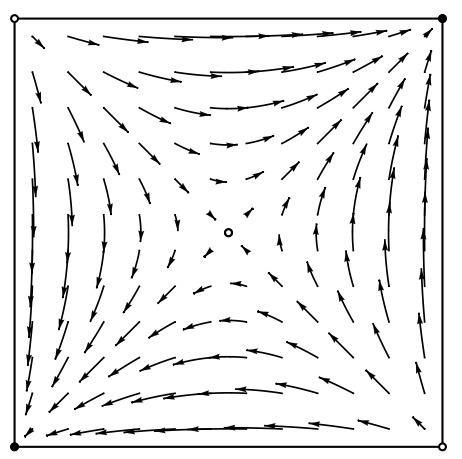
\includegraphics{images/coordination-game.png}
                }
                \subcaption{Response Graph.}
                \label{fig:coordination_game_dynamics}
            \end{minipage}
            \caption{Payoff matrix (a) and Replicator dynamics (b) in the Coordination Game.}
            \label{fig:coordination_game}
        \end{figure}
        %

        \noindent
        To distinguish between recurrent sets and transient points in a dynamical system, the creators of \emph{$\alpha$-Rank} use a complete \emph{Lyapunov function} \cite{lyapunov1950}. This function, $\gamma: X \to \mathbb{R}$, assigns values to points in the space such that:
        %
        \begin{itemize}
            \item For transient points, the value of $\gamma(\phi_t(x))$ strictly decreases over time as the system evolves along the flow $\phi_t$. This reflects how transient points are driven towards the recurrent part of the space.
            \item For points within the recurrent set $\mathcal{R}_\phi$, $\gamma(\phi_t(x))$ remains constant. This signifies that all points within the same chain component share equivalent dynamic properties.
        \end{itemize}
        %

        \noindent
        MCCs offer a discrete-time approximation of the continuous-time dynamics described by \emph{Conley’s Fundamental Theorem}. In the context of MCCs, recurrent sets correspond to SCCs in the response graph, where strategy profiles remain stable over time. On the other hand, transient points are strategy profiles that are not part of any SCCs and eventually escape the system's flow.\tinydouble
        
        \noindent
        The stability of strategy profiles in MCCs is determined by the transition probabilities, similarly to the way the \emph{Lyapunov function} tracks the evolution of a dynamical system. Strategy profiles within a SCC are considered stable because the transition probabilities between them are balanced. This means that, in the SCC, the probability of transitioning from one profile to another is not biased in any particular direction. Each strategy profile has an equal chance of moving to another one within the same SCC. This balance in transition probabilities creates a situation where, once an agent enters the SCC, they are likely to remain within the same set of strategy profiles over time. In contrast, strategy profiles that are not part of any SCC are considered unstable because their transition probabilities are structured in a way that makes moving to a different profile more likely than staying in the current one. This leads them to eventually escape the system's flow.

    \subsubsection{Strategy Evolution Process}

        Given a K-player game, \emph{$\alpha$-Rank} considers the empirical game with K player slots, called $populations$, where individual agents correspond to strategies, i.e. to styles of playing the underlying game. In \emph{$\alpha$-Rank}, populations of agents interact with each other through an evolutionary process following the dynamics of games. The rewards received from these interactions determine how well each strategy performs and, in turn, how often it is adopted by individuals in the populations. Strategies that perform well have a higher probability of being adopted and carried over to the next generation, while those performing poorly are less likely to be adopted. This process of competition and selection between populations leads to their evolution.\tinydouble

        \noindent
        To facilitate evolution, \emph{$\alpha$-Rank} uses the concept of mutation. Initially, populations are monomorphic, meaning all individuals within them choose the same strategy. During K-wise interactions, individuals have a small probability of mutating into different strategies or choosing to stick with their current one. The probability that the mutant will take over the population, defined to be the fixation probability function $\rho$, depends on the relative fitness of the mutant and the population being invaded. Fitness is a function that computes the expected reward an individual can receive when adopting a particular strategy, given the strategies of the other individuals. The stronger the fitness, the more likely it is for individuals to mutate, whereas the lower the fitness, the more likely it is for the mutant to go extinct. When the mutation rate is small, the fitness for any agent $k$ is:
        %
        \begin{equation}
            f^k(str^{k}, str^{-k}) = P^k(str^{k}, str^{-k}),
            \label{eq:fitness_k}
        \end{equation}
        %
        where $P$ represents the empirical game payoff. Formally, the probability of a mutant strategy $str'$ fixating in some population where individuals play strategy $str$ is given by:
        %
        \begin{equation}
            \rho_{str \to str'} = \frac{1 - e^{-\alpha \cdot \Delta f}}{1 - e^{-\alpha \cdot m \cdot \Delta f}} 
            \label{eq:fixation_prob}
        \end{equation}
        %
        assuming that $\Delta f$ is non-zero. $\Delta f = f^k(str', str^{-k}) - f^k(str, str^{-k})$ represents the difference in fitness between the mutant strategy $str'$ and the resident strategy $str$ in the focal population $k$, while the remaining $K - 1$ populations are fixed in their monomorphic strategies $str^{-k}$. Parameter $m$ is the population size and $\alpha$ is the selection intensity. This adjusts the sensitivity of the system to fitness differences: with higher values of $\alpha$, even small differences in fitness lead to larger changes in $\rho$. The nominator measures the potential of the mutant to ``invade'' the resident population solely based on its fitness advantage. Note that, for example, as $\Delta f$ approaches zero, the probability of the mutant's success decreases. The denominator, on the other hand, normalizes the fixation probability using the population size $m$, making it more challenging for a mutant to dominate in larger populations. When $\Delta f$ is zero, the fixation probability equals to $1/m$, indicating that the mutant strategy has the same probability of taking over as any other strategy in the population. This probability is referred to as the \emph{neutral fixation probability}, denoted by $\rho_m$.

    \subsubsection{Modeling Dynamics through MCCs}
    
        In the context of K-player games, \emph{$\alpha$-Rank} creates a Markov transition matrix over strategy profiles. This is an $|\mathcal{S}tr| \times |\mathcal{S}tr|$ matrix that defines the probability of moving from one strategy profile to another based on how likely each population is to change its strategy.
        %
        \begin{eqnarray}
            C_{str \to str'} = 
            \begin{cases} 
                \eta \cdot \rho_{str \to str'} & \text{if } str \neq str' \\ 
                1 - \sum_{str \neq str'} C_{str \to str'} & \text{otherwise}
            \end{cases} 
            \label{eq:transition_matrix_entry}
        \end{eqnarray}
        %

        \noindent
        Here, $C$ is the strategy-transition matrix where each entry $C_{str \to str'}$ represents the probability of transitioning from strategy $str$ to strategy $str'$. The first part of the formula, calculates the probability of transitioning from one strategy to a different one, scaled to ensure that the sum of probabilities for all possible transitions from that strategy sums up to 1. The second part of the formula, computes the probability of staying with the same strategy, $str$, by excluding transitions to all other strategies.\tinydouble

        \noindent
        This evolutionary process of competition and selection among players' strategies leads to a unique stationary probability distribution $\pi$ of dimensionality $|\mathcal{SP}|$, where the mass assigned to a strategy profile indicates how likely it is to resist being ``invaded'' by other strategies as the dynamics evolve. To evaluate and rank strategy profiles —which is the ultimate goal— the method calculates $\pi$ over the game's Markov chain, using the strategy-transition matrix $C$. This distribution indicates how often the system is likely to remain in each profile over time, allowing us to identify the most dominant strategies that are expected to prevail in the long run. Formally, $\pi$ can be computed from the following equation:
        %
        \begin{equation}
            \pi C = \pi \Rightarrow \pi (C - \mathbb{I}) = 0 
            \label{eq:stationary_distribution}
        \end{equation}
        %
        where $\mathbb{I}$ is the identity matrix (see Equation~\ref{eq:c_pi_equation} for the corresponding linear system representation). This means we are looking for a probability vector $\pi$ such that when multiplied by the transition matrix $C$, it remains unchanged. To solve for $\pi$, the augmented matrix from $C - \mathbb{I}$ is constructed and a normalization condition to ensure that probabilities sum to 1 is imposed\footnote{The system $\pi(C - \mathbb{I}) = 0$ by itself does not have a unique solution, as there are infinitely many vectors $\pi$ that satisfy it. To get a unique solution $\pi=(\pi_1,\pi_2,..., \pi_{|\mathcal(SP)|})$, it must hold that $\sum_{i} \pi_i = 1$.}. In this stationary distribution, $\pi=(\pi_1,\pi_2,..., \pi_{|\mathcal(SP)|})$, each $\pi_i$ represents the average time the system spends in strategy profile $i$.
        %
        \begin{equation}
            \begin{bmatrix}
                C_{11} - 1 & C_{12} & \cdots & C_{1n} & | & 0 \\
                C_{21} & C_{22} - 1 & \cdots & C_{2n} & | & 0 \\
                \vdots & \vdots & \ddots & \vdots & | & 0 \\
                C_{n1} & C_{n2} & \cdots & C_{nn} - 1 & | & 0 \\
                1 & 1 & \cdots & 1 & | & 1
            \end{bmatrix}
            \begin{bmatrix}
                \pi_1 \\
                \pi_2 \\
                \vdots \\
                \pi_n \\
                1
            \end{bmatrix}
            =
            \begin{bmatrix}
                0 \\
                0 \\
                \vdots \\
                0 \\
                1
            \end{bmatrix}
        \label{eq:c_pi_equation}
        \end{equation}
        %

\newpage
\subsection{Identifying Strong Joint Policies}

    In this section, we address the challenge of identifying strong joint policies in dynamic games, focusing on strategies that are stable over time and robust to fluctuations. We begin by defining the core problem: how to identify stable joint strategies that persist across multiple iterations of the game. This involves a deeper understanding of how agents’ behaviors evolve and interact within the context of dynamic decision-making. We will present the problem statement that outlines the key challenges in modeling and analyzing strategies in such games.\tinydouble

    \noindent
    Following this, we propose an approach designed to identify and evaluate stable joint strategies in dynamic games. The methodology uses \emph{$\alpha$-Rank} to provide insights into the stability and effectiveness of strategies based on the long-term interactions between agents.

    \subsubsection{Problem Statement}

        In dynamic games, understanding the long-term effect of agents' behaviors is crucial for identifying stable and effective joint strategies. In this context, stability refers to strategies that persist over time—strategies that are robust to fluctuations and deviations. These strategies are considered strong because they are well-aligned with the game’s structure and the agents' payoff expectations during interactions. To identify such stable strategies, one must define and analyze the payoff matrix.\tinydouble
        
        \noindent
        Defining the payoff matrix in static games is relatively straightforward. For example, in Rock-Paper-Scissors, where strategies are individual actions, the payoffs can easily be determined by the game’s rules, such as rock beating scissors (see Table~\ref{tab:rps_payoff}). However, in dynamic games, where policies consist of sequences of actions, defining the payoff matrix is more complex. Even if we manage to estimate payoffs, computing solution concepts like the \emph{Nash equilibrium} can be computationally expensive and may not guarantee convergence, especially in complex or large games. Beyond simply identifying stable joint strategies, it is also crucial to explain why one strategy is better than another. This involves more than just ranking strategies; it requires providing clear evidence for why some strategy profiles are preferred \cite{Vouros_2022}, ensuring transparency in the decision-making process.\tinydouble

        \noindent
        We could, therefore, consider our problem as follows: Given a dynamic game $G$ with $K$ players, our goal is to identify styles of playing $G$, and thus, the set of strategy profiles $\mathcal{SP}$, and rank these profiles based on how stable they are over time, considering long-term agents' interactions towards achieving their objectives. Specifically, we aim to define a ranking function:
        %
        \begin{equation}
            \mathcal{R}: \mathcal{SP} \to \mathbb{R}
            \label{eq:ranking_function}
        \end{equation}
        %
        where $\mathcal{R}(\mathcal{S}_i) > \mathcal{R}(\mathcal{S}_j)$ (resp. $\mathcal{R}(\mathcal{S}_i) \geq \mathcal{R}(\mathcal{S}_j)$) indicates that the strategy profile $\mathcal{S}_i$ is strictly (resp. weakly) preferred over $\mathcal{S}_j$. In conjunction to that, we aim at providing a descriptive framework to promote transparency on how rankings are decided:
        %
        \begin{equation}
            \mathcal{D}: \mathcal{SP} \times \mathcal{SP} \to \mathbb{R}
            \label{eq:descriptive framework}
        \end{equation}
        %

        \noindent
        Empirical game strategies are realized by agents' policies adhering to these strategies in the underlying game. Thus, identifying stable joint strategies in the empirical game translates to identifying stable joint policies adhering to these strategies in the underlying dynamic game.

    \subsubsection{Proposed Methodology}

        To address the challenge of identifying stable joint policies in dynamic games, we propose an approach that combines concepts from \emph{Empirical Game Theory} and \emph{Evolutionary Dynamics}, using \emph{$\alpha$-Rank}, providing transparency to rankings of agent's styles of play.\tinydouble

        \noindent
        Given that the set of agents' policies in dynamic games can be infinitely large we focus on a subset of policies that adhere to concrete and well-defined styles of play. A way to identify styles of play is to observe how players behave in the underlying game or exploit demonstrations of game playing. For instance, human experts performing a task usually follow a distinct set of specific styles based on well-established practices, preferences and experience. Having determined the game playing strategies, we can transform the dynamic game into its empirical form, defining the meta-game by:
        %
        \begin{enumerate}[label=(\alph*)]
            \item Identifying empirical game strategies.
            \item Training policies for agents to play the underlying game according to these strategies.
            \item Defining the empirical game payoff matrix, through simulations, exploiting the trained policies.
        \end{enumerate}
        %

        \noindent
        Once the meta-game is defined, the next step is to define the function $\mathcal{R}$, which ranks joint strategies based on agents' long-term dynamics and objectives. To achieve this, we propose using the evolutionary methodology \emph{$\alpha$-Rank}, which provides rankings by assessing the evolutionary success of each strategy profile. This is reflected in the probability of a given strategy profile being selected over time. This probability is captured by the stationary distribution $\pi$, which is computed by \emph{$\alpha$-Rank} in the limit of infinite ranking intensity $\alpha$. As demonstrated earlier, once $\alpha$ reaches a sufficiently large value, the rankings stabilize, accurately capturing the system's long-term behavior.\tinydouble

        \noindent
        To compute the stationary distribution $\pi$ over strategy profiles, the \emph{$\alpha$-Rank} methodology requires the payoff matrix $P$ of the empirical game. Along with the stationary distribution $\pi$, \emph{$\alpha$-Rank} also outputs the fixation probability function $\rho_{\mathcal{S}_i \to \mathcal{S}_j}$, where $\mathcal{S}_i, \mathcal{S}_j \in \mathcal{SP}$. One could abstractly illustrate \emph{$\alpha$-Rank} as a function:
        %
        \begin{equation}
            \alpha\text{-Rank}(P) \rightarrow (\pi, \rho) 
            \label{eq:abstract_arank}
        \end{equation}
        %

        \noindent
        While the stationary distribution $\pi$ provides valuable insight into the long-term behavior of strategies, it alone does not help us fully understand how strategies transition between one another. The fixation probability function $\rho$, which measures the likelihood of transitioning from one strategy profile $\mathcal{S}_i$ to another $\mathcal{S}_j$, fills this gap. Based on this, the descriptive framework $\mathcal{D}$ can be adequately represented by $\pi$ and $\rho$, which are constituents of the response graph, providing a complete view of the empirical game's dynamics.\tinydouble

        \noindent
        Overall, building on the \emph{$\alpha$-Rank} descriptive framework, the method proposed here for computing strategy profile rankings in dynamic games is as follows:
        %
        \begin{algorithm}
            \caption{Ranking Joint Policies in Dynamic Games}
            \begin{algorithmic}[1]
                \vspace{0.5em}
                \State Identify players' styles of play.
                \State Define the strategies of the empirical game based on those styles.
                \State Train policies realizing the defined strategies.
                \State Run game simulations to create the empirical payoff matrix $P$.
                \State Apply $\alpha$-Rank to define $\mathcal{R}$ and $\mathcal{D}$:
                \vspace{0.5em}
                \State \hspace{1em} Calculate the Markov transition matrix $C$.
                \State \hspace{1em} Find the unique stationary distribution $\pi$.
                \State \hspace{1em} Rank joint strategies by ordering the masses of $\pi$.
                \State \hspace{1em} Describe the rankings through the response graph.
                \State \hspace{1em} Study the effect of different $\alpha$ values on $\pi$.
            \end{algorithmic}
        \end{algorithm}
        %

\newpage
\subsection{Identifying Strong Joint Policies}

\begin{flushleft}


    \subsubsection{Problem Statement}

    \begin{flushleft}

        In dynamic games, understanding the long-term effect of agents' behaviors is crucial for identifying stable and effective joint strategies. In this context, stability refers to strategies that persist over time—strategies that are robust to fluctuations and deviations. These strategies are considered strong because they are well-aligned with the game’s structure and the agents' payoff expectations during interactions. To identify such stable strategies, one must define and analyze the payoff matrix.\\~\\
        
        Defining the payoff matrix in static games is relatively straightforward. For example, in Rock-Paper-Scissors, where strategies are individual actions, the payoffs can easily be determined by the game’s rules, such as rock beating scissors (see Table~\ref{tab:rps_payoff}). However, in dynamic games, where policies consist of sequences of actions, defining the payoff matrix is more complex. Even if we manage to estimate payoffs, computing solution concepts like the \emph{Nash equilibrium} can be computationally expensive and may not guarantee convergence, especially in complex or large games. Beyond simply identifying stable joint strategies, it is also crucial to explain why one strategy is better than another. This involves more than just ranking strategies; it requires providing clear evidence for why some strategy profiles are preferred, ensuring transparency in the decision-making process.\\~\\

        We could, therefore, consider our problem as follows: Given a dynamic game $G$ with $K$ players, our goal is to identify styles of playing $G$, and thus, the set of strategy profiles $\mathcal{SP}$, and rank these profiles based on how stable they are over time, considering long-term agents' interactions towards achieving their objectives. Specifically, we aim to define a ranking function:
        %
        \begin{equation}
            \mathcal{R}: \mathcal{SP} \to \mathbb{R}
            \label{eq:ranking_function}
        \end{equation}
        %
        
        where $\mathcal{R}(\mathcal{S}_i) > \mathcal{R}(\mathcal{S}_j)$ (resp. $\mathcal{R}(\mathcal{S}_i) \geq \mathcal{R}(\mathcal{S}_j)$) indicates that the strategy profile $\mathcal{S}_i$ is strictly (resp. weakly) preferred over $\mathcal{S}_j$, using a descriptive framework that provides transparency on how rankings are decided:
        %
        \begin{equation}
            \mathcal{D}: \mathcal{SP} \times \mathcal{SP} \to \mathbb{R}
            \label{eq:descriptive framework}
        \end{equation}
        %

        Empirical game strategies are realized by agents' policies adhering to these strategies in the underlying game. Thus, identifying stable joint strategies in the empirical game translates to identifying stable joint policies adhering to these strategies in the underlying dynamic game.

    \end{flushleft}

    \subsubsection{Proposed Methodology}

    \begin{flushleft}

        To address the challenge of identifying stable joint policies in dynamic games, we propose an approach that combines concepts from \emph{Empirical Game Theory} and \emph{Evolutionary Dynamics}, using \emph{$\alpha$-Rank}, providing transparency to rankings of agent's styles of play.\\~\\

        Given that the set of agents' policies in dynamic games can be infinitely large we focus on a subset of policies that adhere to concrete and well-defined styles of play. A way to identify styles of play is to observe how players behave in the underlying game or exploit demonstrations of game playing. For instance, human experts performing a task usually follow a distinct set of specific styles based on well-established practices, preferences and experience. Having determined the game playing strategies, we can transform the dynamic game into its empirical form, defining the meta-game by:
        %
        \begin{enumerate}[label=(\alph*)]
            \item Identifying empirical game strategies.
            \item Training policies for agents to play the underlying game according to these strategies.
            \item Defining the empirical game payoff matrix, through simulations, exploiting the trained policies.
        \end{enumerate}
        %

        Once the meta-game is defined, the next step is to define the function $\mathcal{R}$, which ranks joint strategies based on agents' long-term dynamics and objectives. To achieve this, we propose using the evolutionary \emph{$\alpha$-Rank} methodology, which determines rankings by assessing the evolutionary success of each strategy profile. This success is reflected in the probability of a given strategy profile being selected over time. This probability is captured by the stationary distribution $\pi$, which is computed by \emph{$\alpha$-Rank} in the limit of infinite ranking intensity $\alpha$. As demonstrated by \cite{omidshafiei2019alpharank}, once $\alpha$ reaches a sufficiently large value, the rankings stabilize, accurately capturing the system's long-term behavior.

        To compute the stationary distribution $\pi$ over strategy profiles, the \emph{$\alpha$-Rank} methodology requires the payoff matrix $P$ of the empirical game. Along with the stationary distribution $\pi$, \emph{$\alpha$-Rank} also outputs the fixation probability function $\rho_{\mathcal{S}_i \to \mathcal{S}_j}$, where $\mathcal{S}_i, \mathcal{S}_j \in \mathcal{SP}$. One could abstractly illustrate \emph{$\alpha$-Rank} as a function:
        %
        \begin{equation}
            \alpha\text{-Rank}(P) \rightarrow (\pi, \rho) 
            \label{eq:abstract_arank}
        \end{equation}
        %

        While the stationary distribution $\pi$ provides valuable insight into the long-term behavior of strategies, it alone does not help us fully understand how strategies transition between one another. The fixation probability function $\rho$, which measures the likelihood of transitioning from one strategy profile $\mathcal{S}_i$ to another $\mathcal{S}_j$, fills this gap. Based on this, the descriptive framework $\mathcal{D}$ can be adequately represented by $\pi$ and $\rho$, which are constituents of the response graph, which provides a complete view of the empirical game dynamics.\\~\\

        Overall, building on the \emph{$\alpha$-Rank} descriptive framework, the method proposed here for computing strategy profile rankings in dynamic games is as follows:
        %
        \begin{algorithm}
            \caption{Ranking Joint Policies in Dynamic Games}
            \begin{algorithmic}[1]
                \vspace{0.5em}
                \STATE Identify players' styles of play.
                \STATE Define the strategies of the empirical game based on those styles.
                \STATE Train policies realizing the defined strategies.
                \STATE Run game simulations to create the empirical payoff matrix $P$.
                \STATE Apply \emph{$\alpha$-Rank} to define $\mathcal{R}$ and $\mathcal{D}$:
                \vspace{0.5em}
                \STATE \hspace{1em} Calculate the Markov transition matrix $C$.
                \STATE \hspace{1em} Find the unique stationary distribution $\pi$.
                \STATE \hspace{1em} Rank joint strategies by ordering the masses of $\pi$.
                \STATE \hspace{1em} Describe the rankings through the response graph.
                \STATE \hspace{1em} Study the effect of different $\alpha$ values on $\pi$.
            \end{algorithmic}
        \end{algorithm}
        %

    \end{flushleft}

\end{flushleft}

\newpage
\subsection{Identifying Strong Joint Policies in the GCG}

    In this section, we apply our methodology to the \emph{Graph Coloring Game} (GCG) defined in Section~\ref{sec:2.1}, to identify strong joint policies. This analysis allows us to provide an explainable link between the observed policies and the actions they refer to.\tinydouble

    \noindent
    We begin by defining the different styles of play and modeling them as policies using \emph{neural network} (NN) models. Next, we define the empirical game payoff matrix, which measures how well these policies interact with each other over the long run. Finally, we apply \emph{$\alpha$-Rank} to evaluate and rank the joint policies, gaining insights into the game's dynamics.

    \subsubsection{Defining Styles of Play}
    \label{sec:5.1}

        The process of transforming the underlying dynamic GCG into its empirical form begins by understanding the different ways in which agents play the game. This involves two essential steps:
        %
        \begin{enumerate}
            \item Identifying agents' strategies.
            \item Constructing the empirical game payoff matrix.
        \end{enumerate}
        %

        \noindent
        Agents' strategies in the game can be thought of as different styles of play, which are typically revealed through preferences and behaviors in response to the game’s structure. In our experiments, we specify different styles across three main dimensions: color tone (preference for which colors to use), block difficulty (preference for the types of blocks to choose), and coloring approach (preference for the number of colors to use), as shown in Table~\ref{tab:preferences}. These dimensions are combined to define a player's overall style, which can range from complete indifference—where no specific preference is observed in any of the dimensions (denoted by "I")—to highly specific preferences across all dimensions.
        %
        \begin{table}[H]
            \centering
            \caption{Dimensions specifying agents' strategies.}
            \label{tab:preferences}
            \vspace{0.5em}
            \begin{tabular}{ll}
                \toprule
                \textit{Preference Dimension} & \textit{Value} \\ 
                \midrule
                Color Tone & warm (W) vs. cool (C) \\ 
                Block Coloring Difficulty & small (L) vs. large (A) \\ 
                Coloring Approach & minimalistic (M) vs. extravagant (E) \\ 
                \bottomrule
            \end{tabular}
        \end{table}
        %

    \subsubsection{Realizing the Empirical Game Strategies}

        Policies corresponding to specific strategies are realized using \emph{convolutional neural networks} (CNNs), which are trained to adapt to different styles of play in the GCG. To guide the training of these policies, we assign specific values to each of the three dimensions of the game's \emph{preference reward} —color tone, block difficulty, and coloring approach. These values, range from -1 to 1, where 1 indicates a strong preference for a particular dimension. For example, a value of 0.7 for warm colors suggests a relatively strong preference for warm tones, while values closer to 0 a tendency towards indifference.\tinydouble
        
        \noindent
        In our experimental setting, we define a total of 11 distinct styles of play: I, C, W, E, M, L, A, AE, CA, LE and WL, given ``I'' and combinations of preference values specified in Table~\ref{tab:preferences}. Assuming no inherent bias among the players of the empirical game, we allow populations to sample from the same list of strategies.\tinydouble

        \noindent
        All the policy models used to realize the empirical game strategies share a common underlying architecture and training setup. Although hyperparameter tuning is typically recommended, it doesn't make much difference in this case, as these models are relatively easy to optimize when trained in small settings. Regarding the CNN architecture, it consists of four convolutional layers, each defined with a kernel size of 3, stride of 1, and padding of 1. These parameters are chosen to ensure that the model is capable of extracting spatial features from the input data, which in this case is a grid representation of the game state. 
        %
        \begin{figure}[H]
            \centering
            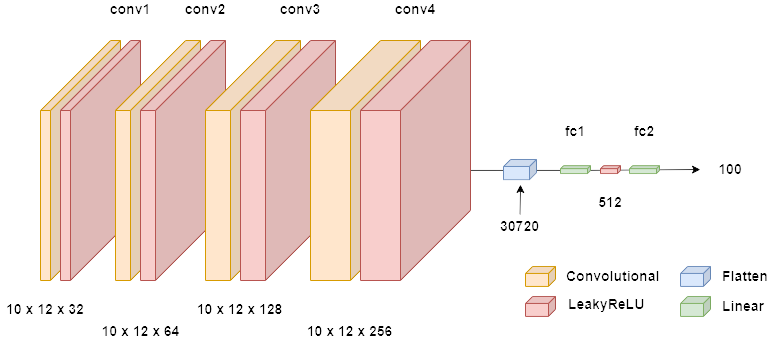
\includegraphics[width=0.9\linewidth]{images/convDQN.png}
            \caption{Convolution Policy Network Architecture.}
            \label{fig:convDQN}
        \end{figure}
        %
        
        \noindent
        The input tensor has dimensions $10 \times 12$, where $|B|=10$ represents the number of blocks in the state and $|CR^*|=12$ represents the number of possible colors a block can have. Each block is encoded using one-hot encoding, meaning that each color is represented as a binary vector of length 12. The output is then flattened and passed through two \emph{fully connected} (FC) layers, which process the data to produce the final output, as shown in Figure~\ref{fig:convDQN}.\tinydouble

        \noindent
        Policy models are trained individually in the underlying game using the deep Q-learning reinforcement learning algorithm specified in Algorithm~\ref{alg:dqn_algorithm}. We set $\gamma$ to 0.7. To optimize the model parameters, we use the smooth L1 loss function with $\beta$=1.0 and the Adam optimizer with a learning rate of 5e-4 and weight decay of 1e-5 to prevent over-fitting. To further enhance the learning process, we incorporate experience replay, with a memory that stores up to 10 million experiences \cite{10.1007/BF00992699}. A target network alongside the main policy network, is being used according to the \emph{Double-DQN} approach \cite{vanhasselt2015deep}. To update the target network we apply a soft update with a factor $\tau$=5e-3. This gradually brings the target network closer to the policy network, balancing learning speed and stability. With a batch size of 64, we train the models for 10,000 episodes.
        %
        \begin{algorithm}
            \caption{Double Deep Q-Learning with Experience Replay}
            \label{alg:dqn_algorithm}
            \begin{algorithmic}[1]
            \State $Q_\theta$, $Q_{\theta'} \gets Q_\theta$, $M$ \Comment{Initialize policy/target nets \& memory}
            \For{episode}
                \State $s \gets s_{0}$
                \For{step}
                    \State $a \gets \text{argmax}_a Q_\theta(s)$ \Comment{Select $\epsilon$-greedy action}
                    \State $(s, a, r, s') \in M$ \Comment{Store experience}
                    \If{$|M| > \text{batch size}$} 
                        \For{each $(s, a, r, s')$ in $M$} \Comment{Sample memory}
                            \State $y \gets r + \gamma \max_{a'} Q_{\theta'}(s')$
                            \State $L \gets \text{Loss}(Q_\theta(s), y)$
                            \State $\theta \gets \theta - \alpha \nabla_\theta L$
                        \EndFor
                    \EndIf
                    \State $Q_{\theta'} \gets \tau Q_\theta + (1 - \tau) Q_{\theta'}$ \Comment{Soft update}
                    \State $s \gets s'$
                \EndFor
            \EndFor
            \end{algorithmic}
        \end{algorithm}
        %

        \noindent
        In this setup, the agents are trained without any co-players, meaning that each model learns in isolation. This approach is intentional, as our goal is to develop agents that play optimally on their own, rather than in collaboration with others. The idea is to explore how different styles of independent players interact with each other. We expect that some styles will lead to more conflicts than others, and this behavior is key to our analysis. If we had trained the agents together, for example using a \emph{multi-agent reinforcement learning} (MARL) approach designed for collaborative settings, the resulting agents would have learned joint policies, which would defeat the very purpose of evaluating how their individual  policies affect collaboration.\tinydouble

        \noindent
        Let us consider, for instance, the simulation statistics of two relatively compatible play styles that we expect to perform well together in the game: Player W (a robot player with preferences for warm color tones) and player C (a human with preferences for cool color tones). In Figure~\ref{fig:cw-solution}, we observe how these players' individual preferences shape their interactions.
        %
        \begin{figure}[H]
            \centering
            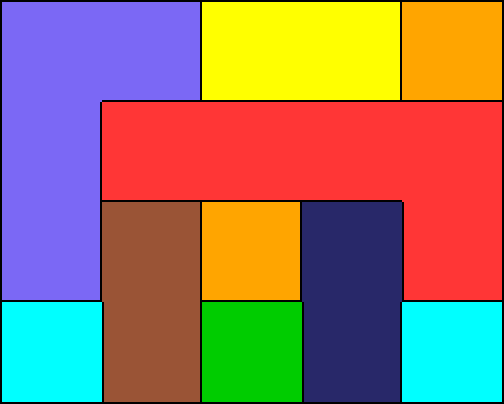
\includegraphics[width=0.5\textwidth]{images/cw-solution.png}
            \caption{Example solution to the game showing how C player and W player interact based on their preferences.}
            \label{fig:cw-solution}
        \end{figure}
        %
        
        \noindent
        The statistics in Figure~\ref{fig:cw-stats} reveal the most frequently selected actions in terms of blocks and colors. Player C prefers colors like blue, purple, and green, while player W tends to choose colors like brown, orange, and red. Given these preferences, conflicts are unlikely to arise from color selection alone. Even in scenarios where they may choose to color neighboring blocks, it is highly impossible that both players will choose the same color.
        %
        \begin{figure}[H]
            \centering
            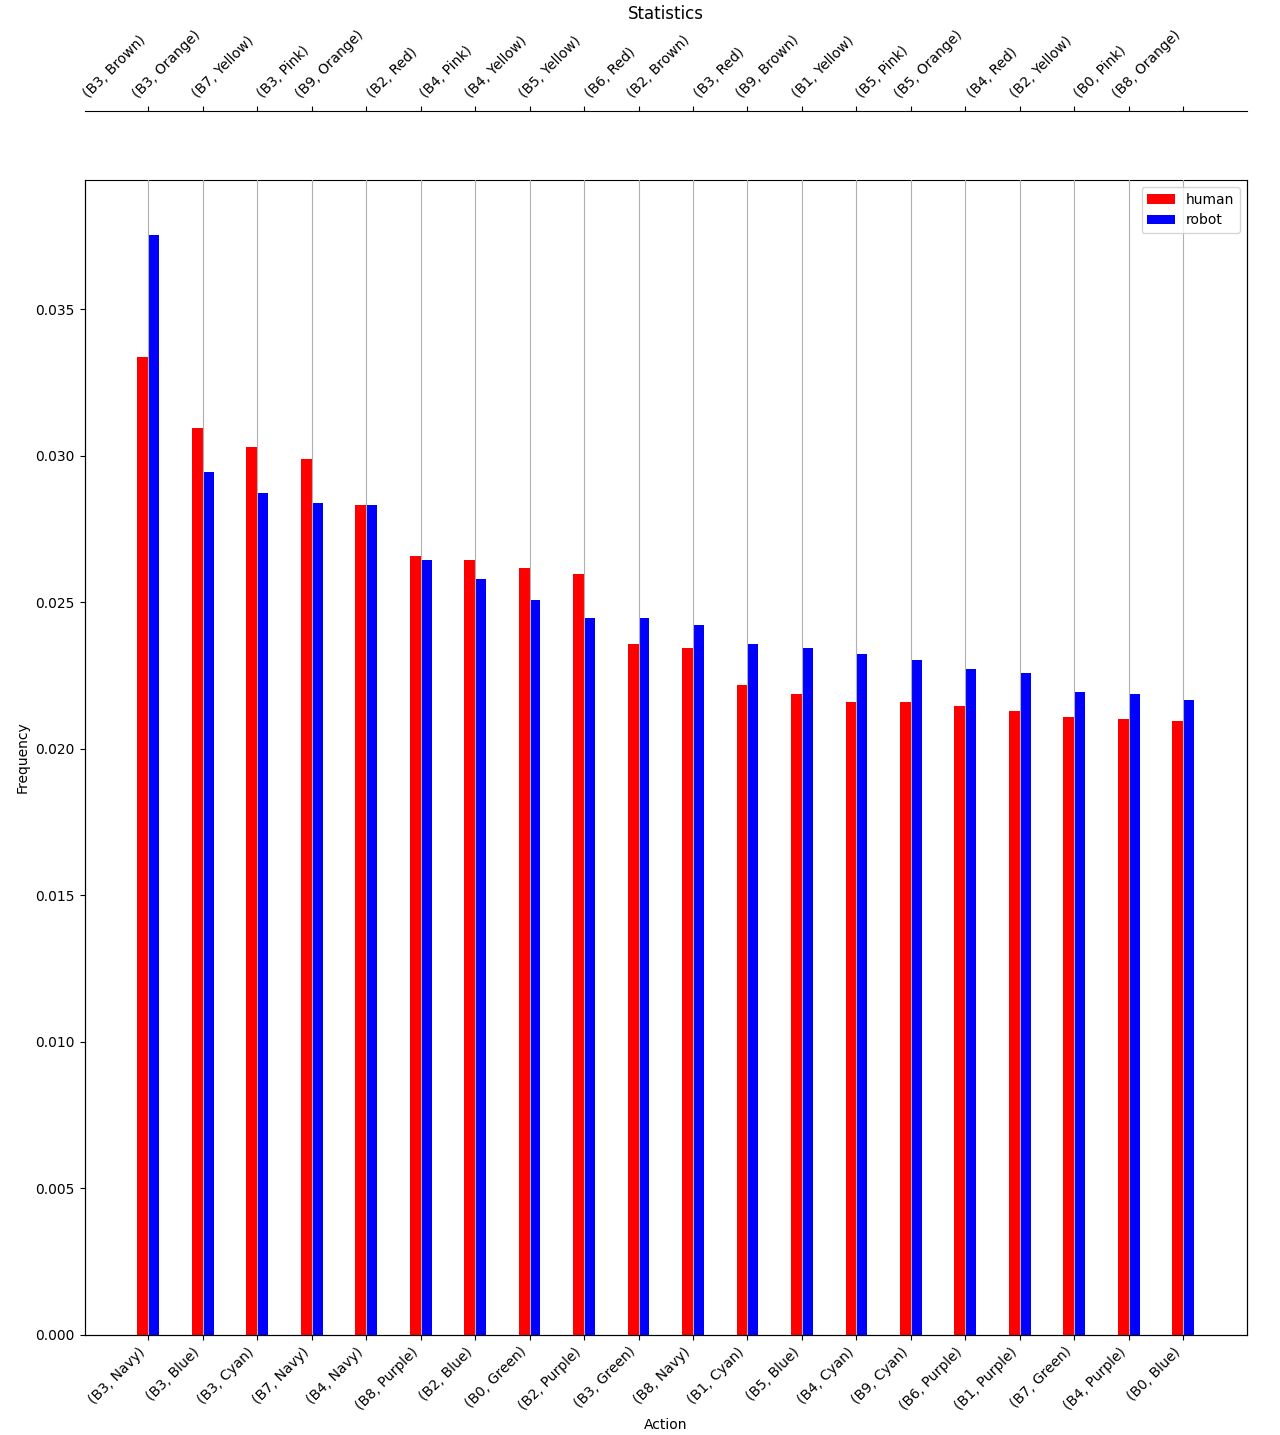
\includegraphics[width=0.9\textwidth]{images/cw-stats.png}
            \caption{Statistical analysis of the most frequently selected actions by C player and W player.}
            \label{fig:cw-stats}
        \end{figure}
        %        

        \noindent
        On the other hand, in Figure~\ref{fig:cc-solution}, we observe the interactions between two C players. In this case, we expect more conflicts, as both players share similar color preferences. This increases the likelihood of both players selecting the same color for neighboring blocks.
        %
        \begin{figure}[H]
            \centering
            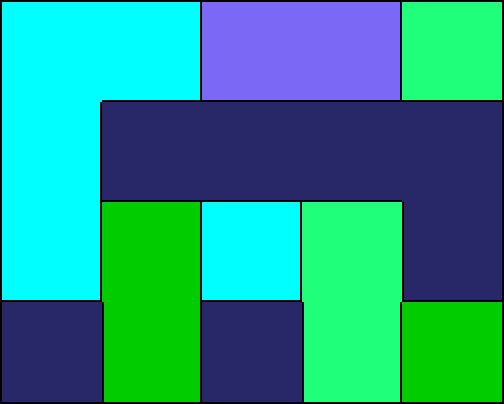
\includegraphics[width=0.5\textwidth]{images/cc-solution.png}
            \caption{Example solution to the game showing how two C players interact based on their preferences.}
            \label{fig:cc-solution}
        \end{figure}
        %
        
        \noindent
        The statistics shown in in Figure~\ref{fig:cc-stats} further support this, as they reveal a high probability of color overlap, primarily due to the dominance of cool colors in both action spaces. However, these conflicts are not a result of insufficient training, but rather stem from the inherent similarity in preferences.
        %
        \begin{figure}[H]
            \centering
            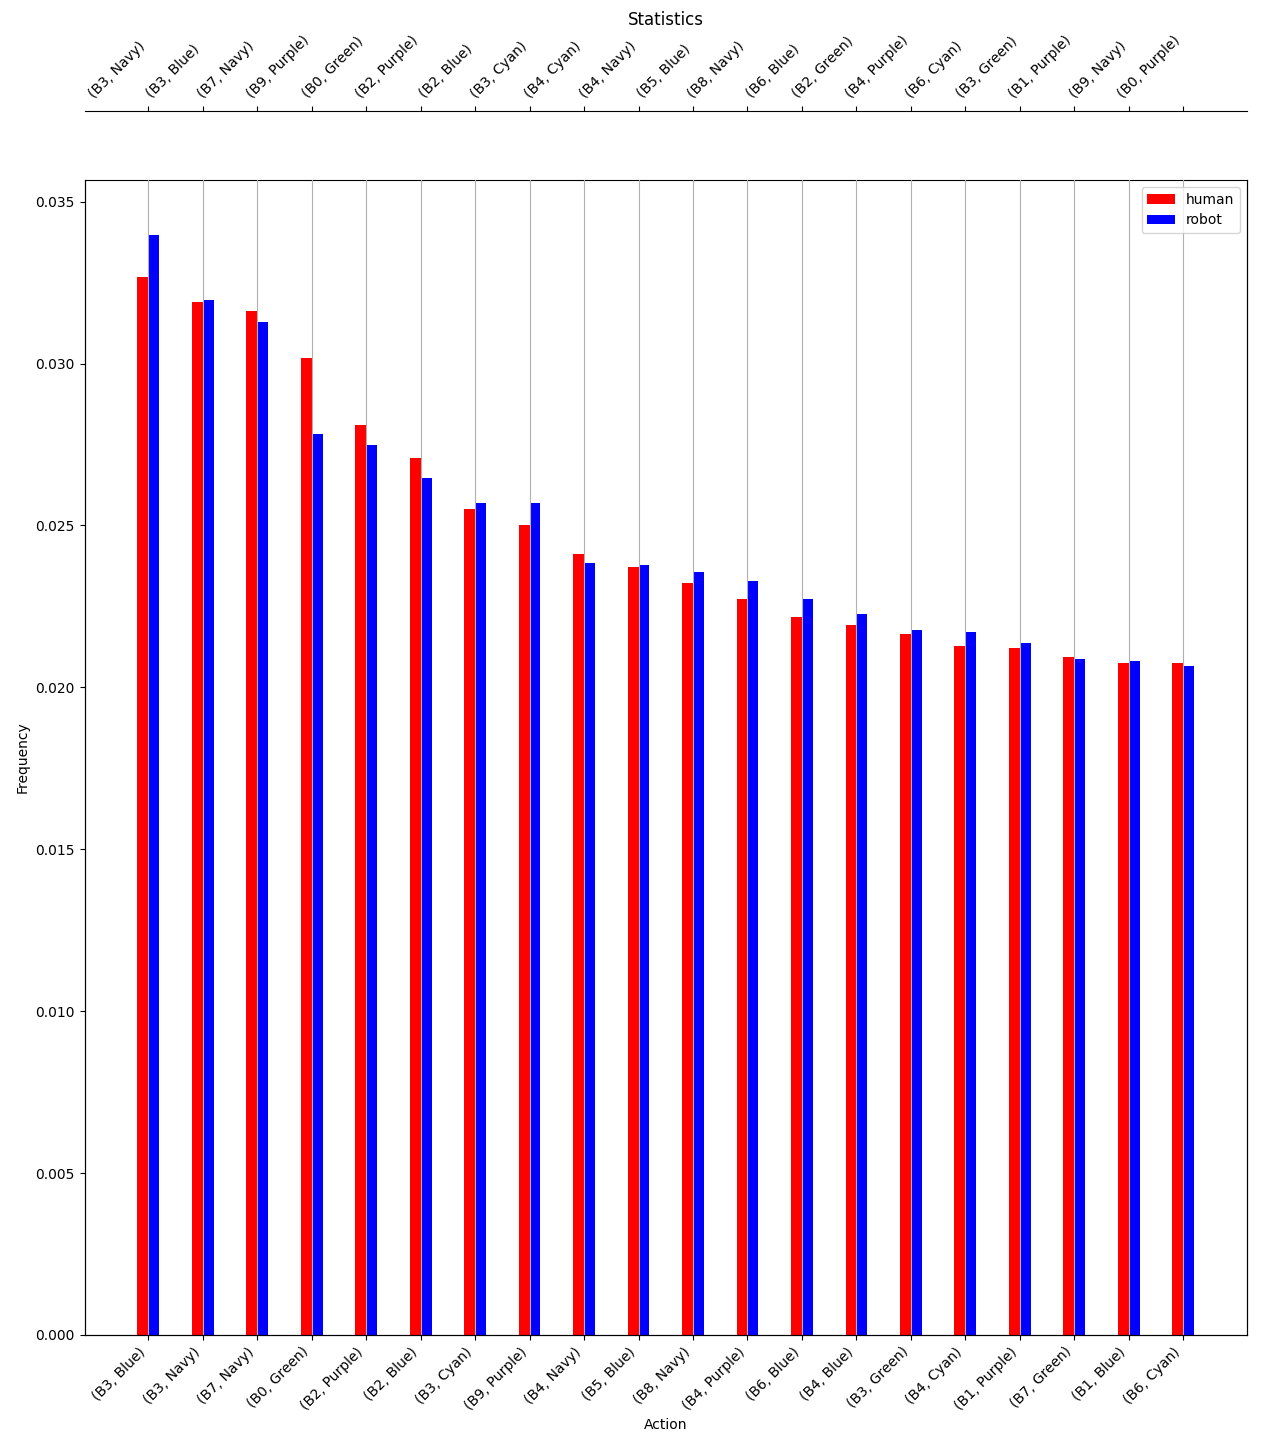
\includegraphics[width=0.9\textwidth]{images/cc-stats.png}
            \caption{Statistical analysis of the most frequently selected actions by two C players.}
            \label{fig:cc-stats}
        \end{figure}
        %   

        \noindent
        Other than that, both agents have been thoroughly trained in isolation, exploring a wide range of states and ultimately converging to stable policies. This allows them to respond effectively and optimally, even when paired with agents with conflicting styles of play. Therefore, even in the case of the most incompatible pairings, the number of mistakes remains minimal, and these mistakes are not due to inadequate exploration, but rather to the inherent conflicts in the agents’ preferences. 

    \subsubsection{Extracting the Empirical Payoff Matrix}

        We generate the empirical payoff matrix by simulating each strategy profile over multiple games. These payoffs represent how well different styles of play perform jointly, according to the game’s rules.\tinydouble

        \noindent
        The values in the payoff matrix are computed in terms of the delay and the quality of the solution according to the game's constraints (gain, penalty, and sanction), excluding preferences. This ensures a common ground for distinct strategies, evaluating solutions solely based on the game's rules. For each pair of strategies, we simulate the game over 5,000 repeats and calculate the average payoff for each strategy. These values are then organized into the payoff matrix, which is provided in Table~\ref{tab:gcg_payoff_matrix}. Each entry in the matrix represents the payoffs of strategies in the corresponding profile, with the first value indicating the payoff of the row player and the second value of the column player. The Nash equilibria are highlighted in bold, while nine of the top-ranked strategy profiles in the MCC are shaded in gray.
        %
        \begin{table}[h!]
            \centering
            \caption{Empirical Payoff Matrix for the Graph Coloring Game.}
            \label{tab:gcg_payoff_matrix}
            \vspace{0.5em}
            \resizebox{\textwidth}{!}{%
            \begin{tabular}{lccccccccccc}
                \hline
                    & A & AE & C & CA & E & I & L & LE & M & W & WL \\
                \hline
                A  & (3.12, 3.11) & (3.15, 3.16) & (3.17, 3.17) & (3.14, 3.17) & (3.16, 3.17) & (3.16, 3.15) & (3.22, 3.13) & (3.19, 3.16) & (3.15, 3.18) & (3.16, 3.17) & (3.21, 3.18) \\
                
                AE & (3.17, 3.17) & (3.11, 3.11) & (3.18, 3.17) & \cellcolor{gray!16}(3.15, 3.17) & (3.17, 3.16) & (3.19, 3.16) & (3.23, 3.12) & (3.19, 3.16) & \cellcolor{gray!16}(3.15, 3.18) & (3.17, 3.17) & (3.20, 3.16) \\
                
                C  & (3.17, 3.16) & (3.16, 3.17) & (3.10, 3.10) & (3.14, 3.17) & (3.15, 3.15) & (3.18, 3.15) & (3.22, 3.12) & (3.17, 3.14) & (3.14, 3.17) & (3.17, 3.16) & (3.20, 3.17) \\
                
                CA & (3.17, 3.15) & (3.17, 3.15) & (3.17, 3.14) & (3.11, 3.11) & (3.18, 3.15) & (3.18, 3.14) & (3.24, 3.13) & \cellcolor{gray!16}(3.21, 3.16) & \cellcolor{gray!16}(3.16, 3.16) & (3.19, 3.16) & \cellcolor{gray!16}(3.22, 3.15) \\
                
                E  & (3.15, 3.16) & (3.16, 3.16) & (3.15, 3.16) & \cellcolor{gray!16}(3.15, 3.17) & (3.10, 3.10) & (3.18, 3.16) & (3.22, 3.12) & (3.19, 3.14) & (3.15, 3.17) & (3.16, 3.17) & (3.19, 3.17) \\
                
                I  & (3.14, 3.16) & (3.16, 3.18) & (3.16, 3.18) & (3.15, 3.19) & (3.16, 3.17) & (3.12, 3.12) & (3.22, 3.14) & (3.18, 3.16) & (3.14, 3.19) & (3.16, 3.18) & (3.19, 3.18) \\

                L  & (3.14, 3.22) & (3.11, 3.22) & (3.12, 3.22) & (3.13, 3.23) & (3.12, 3.22) & (3.13, 3.22) & (3.12, 3.12) & (3.14, 3.20) & (3.11, 3.21) & (3.14, 3.23) & \textbf{(3.15, 3.21)} \\
                
                LE & (3.15, 3.19) & (3.14, 3.18) & (3.14, 3.18) & (3.15, 3.21) & (3.15, 3.19) & (3.16, 3.17) & (3.20, 3.14) & (3.11, 3.11) & (3.14, 3.22) & (3.15, 3.18) & (3.18, 3.19) \\
                
                M  & (3.17, 3.14) & (3.17, 3.15) & (3.17, 3.15) & \cellcolor{gray!16}(3.16, 3.17) & (3.16, 3.14) & (3.18, 3.14) & (3.23, 3.11) & (3.20, 3.14) & (3.06, 3.08) & (3.18, 3.15) & (3.20, 3.16) \\
                
                W  & (3.17, 3.17) & (3.17, 3.18) & (3.16, 3.18) & \cellcolor{gray!16}(3.16, 3.20) & (3.17, 3.17) & (3.18, 3.16) & (3.21, 3.13) & (3.18, 3.15) & (3.15, 3.18) & (3.08, 3.09) & (3.19, 3.15) \\
            
                WL & (3.17, 3.20) & (3.17, 3.19) & (3.17, 3.19) & (3.17, 3.22) & (3.17, 3.19) & (3.18, 3.19) & \textbf{(3.21, 3.15)} & (3.19, 3.17) & \cellcolor{gray!16}(3.16, 3.20) & (3.16, 3.19) & (3.13, 3.13) \\
                \hline
            \end{tabular}
            }
        \end{table}
        %

        \noindent
        From this matrix, we observe that (L, WL) and its symmetric counterpart (WL, L) both with payoffs of (3.15, 3.21) and (3.21, 3.15) respectively, are the only Nash equilibria. It is important to note here that these equilibria prescribe agents' strategies given that they do play the game with rational co-players, but they do not capture the overall dynamics of the game, considering the long-term effects of agents' interactions.

    \subsubsection{Evaluating and Ranking Joint Policies}

        Given the payoff matrix derived from the empirical analysis, we apply the \emph{$\alpha$-Rank} method to evaluate the performance of strategy profiles over time in terms of the MCC solution concept. Specifically, we ran the method 1,000 times, using values of $\alpha$ within the range $[0.1, 10]$ with step=0.01, while assuming populations of size $m=100$. We provide as input the strategies defined in Section~\ref{sec:5.1} and the empirical game payoff matrix. We focus on the rankings of the top 6 strategy profiles, to identify the stronger ones across different values of $\alpha$.\tinydouble

        \noindent
        As we observe from the rankings in Table~\ref{tab:ranking_table}, the strategy profile that prevails in the long run is (WL, CA); this is the primary component of the MCC. Although the table was derived using an $\alpha$ value of 2, the rankings remain consistent even when $\alpha$ is set to 10. We choose $\alpha=2$ over $\alpha=10$, to display the rankings of lower-performing strategy profiles, which would otherwise drop to zero. First, it is worth mentioning that the Nash equilibria (L, WL) and (WL, L) don't appear among the top-ranked strategy profiles. This is because MCC components are defined based on how well strategies perform when interacting with other strategies, based on long-term agents interactions. The individual strategies within the Nash equilibrium profile, either WL or L, may not result in favorable interactions with other strategies. As a result, the profile (WL, L) is ranked lower that others.
        %
        \begin{table}[H]
            \centering
            \caption{Rankings for $\alpha=2$.}
            \label{tab:ranking_table}
            \vspace{0.5em}
            \begin{tabular}{lcc}
                \hline
                \textbf{Agent} & \textbf{Rank} & \textbf{Score} \\
                \hline
                (WL, CA) & 1 & 0.42 \\
                (W, CA) & 2 & 0.13 \\
                (M, CA) & 3 & 0.12 \\
                (CA, M) & 4 & 0.08 \\
                (CA, W) & 5 & 0.08 \\
                (CA, LE) & 6 & 0.01 \\
                \hline
            \end{tabular}
        \end{table}
        %

        \noindent
        To further support our observations regarding the misalignment between the two solution concepts, let's examine why (CA, WL) is part of the MCCs, while (L, WL), the Nash equilibrium, is not. A closer look at the payoff matrix in Table~\ref{tab:gcg_payoff_matrix} reveals that L appears to be the worst-performing strategy for the row player, with an average payoff of 3.13. In this case, being in the Nash equilibrium means the player is stuck with a strategy that gives low rewards, making it the best among other options, rather than a strong choice. If it happens to play this strategy, it would expect its rational opponent to play WL. Strategy CA on the other hand, is the best-performing strategy for the row player, with an average payoff of 3.18. Combined with WL, which is the best performing strategy for the column player, with an average payoff of 3.18, they make profile (CA, WL) becomes the top ranked strategy profile in the ranking Table~\ref{tab:ranking_table}.\tinydouble

        \noindent
        Rankings within the MCC are also very intuitive. For example, strategies that prefer different color tones, such as (WL, CA) or (W, CA), tend to result into fewer conflicts since, they naturally avoid selecting the same colors. Similarly, strategies that prefer different blocks based on their difficulty, such as (WL, CA) or (CA, LE), tend to provide solutions with minimal delay, as they naturally avoid coloring the same blocks. Notably, profiles with mixed preferences across these dimensions demonstrate the most promising performance, which explains why (WL, CA), as such a profile, is a key component of the MCC. However, not all profile rankings can be easily explained through the game's rules alone; the expected influence of certain strategies on the quality of the solutions remains ambiguous. For example, profiles with strategies like M and E are more difficult to analyze.
        %
        \begin{figure}[H]
            \centering
            \begin{subfigure}[b]{0.45\linewidth}
                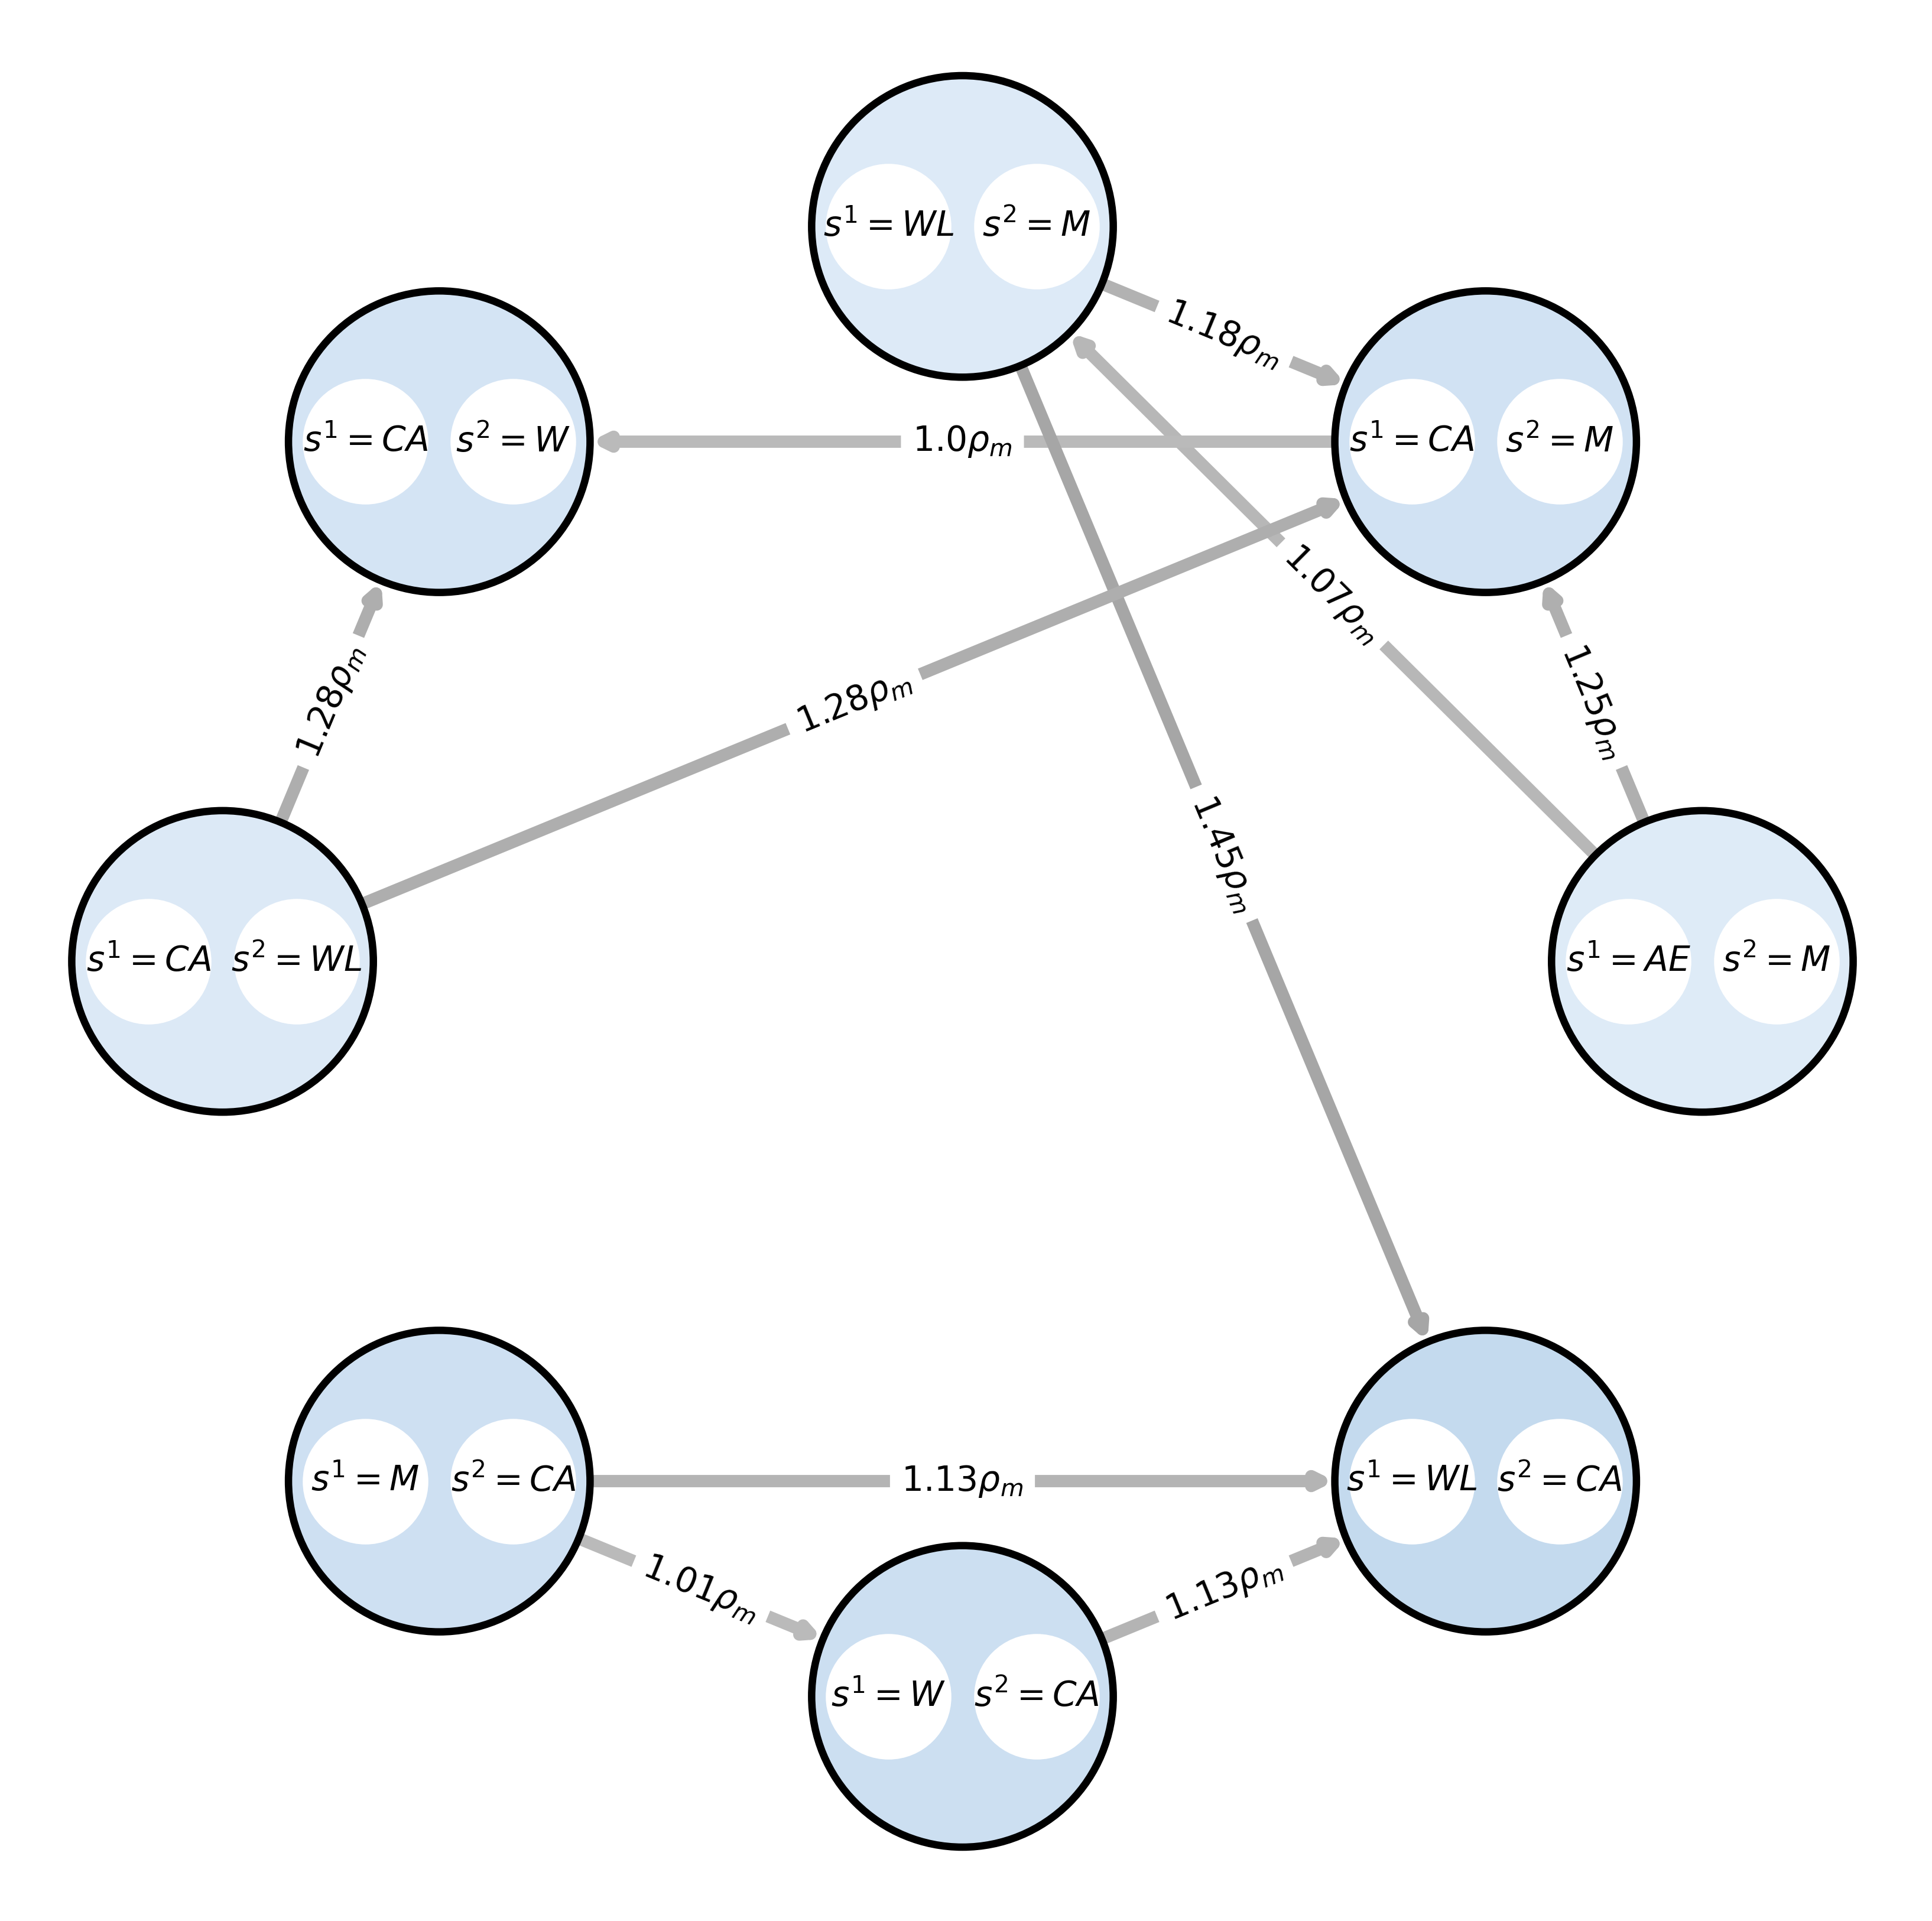
\includegraphics[width=\linewidth]{images/rg_0.4.png}
                \caption{$alpha=0.4$}
                \label{fig:response_graph_0.4}
            \end{subfigure}
            \hfill
            \begin{subfigure}[b]{0.45\linewidth}
                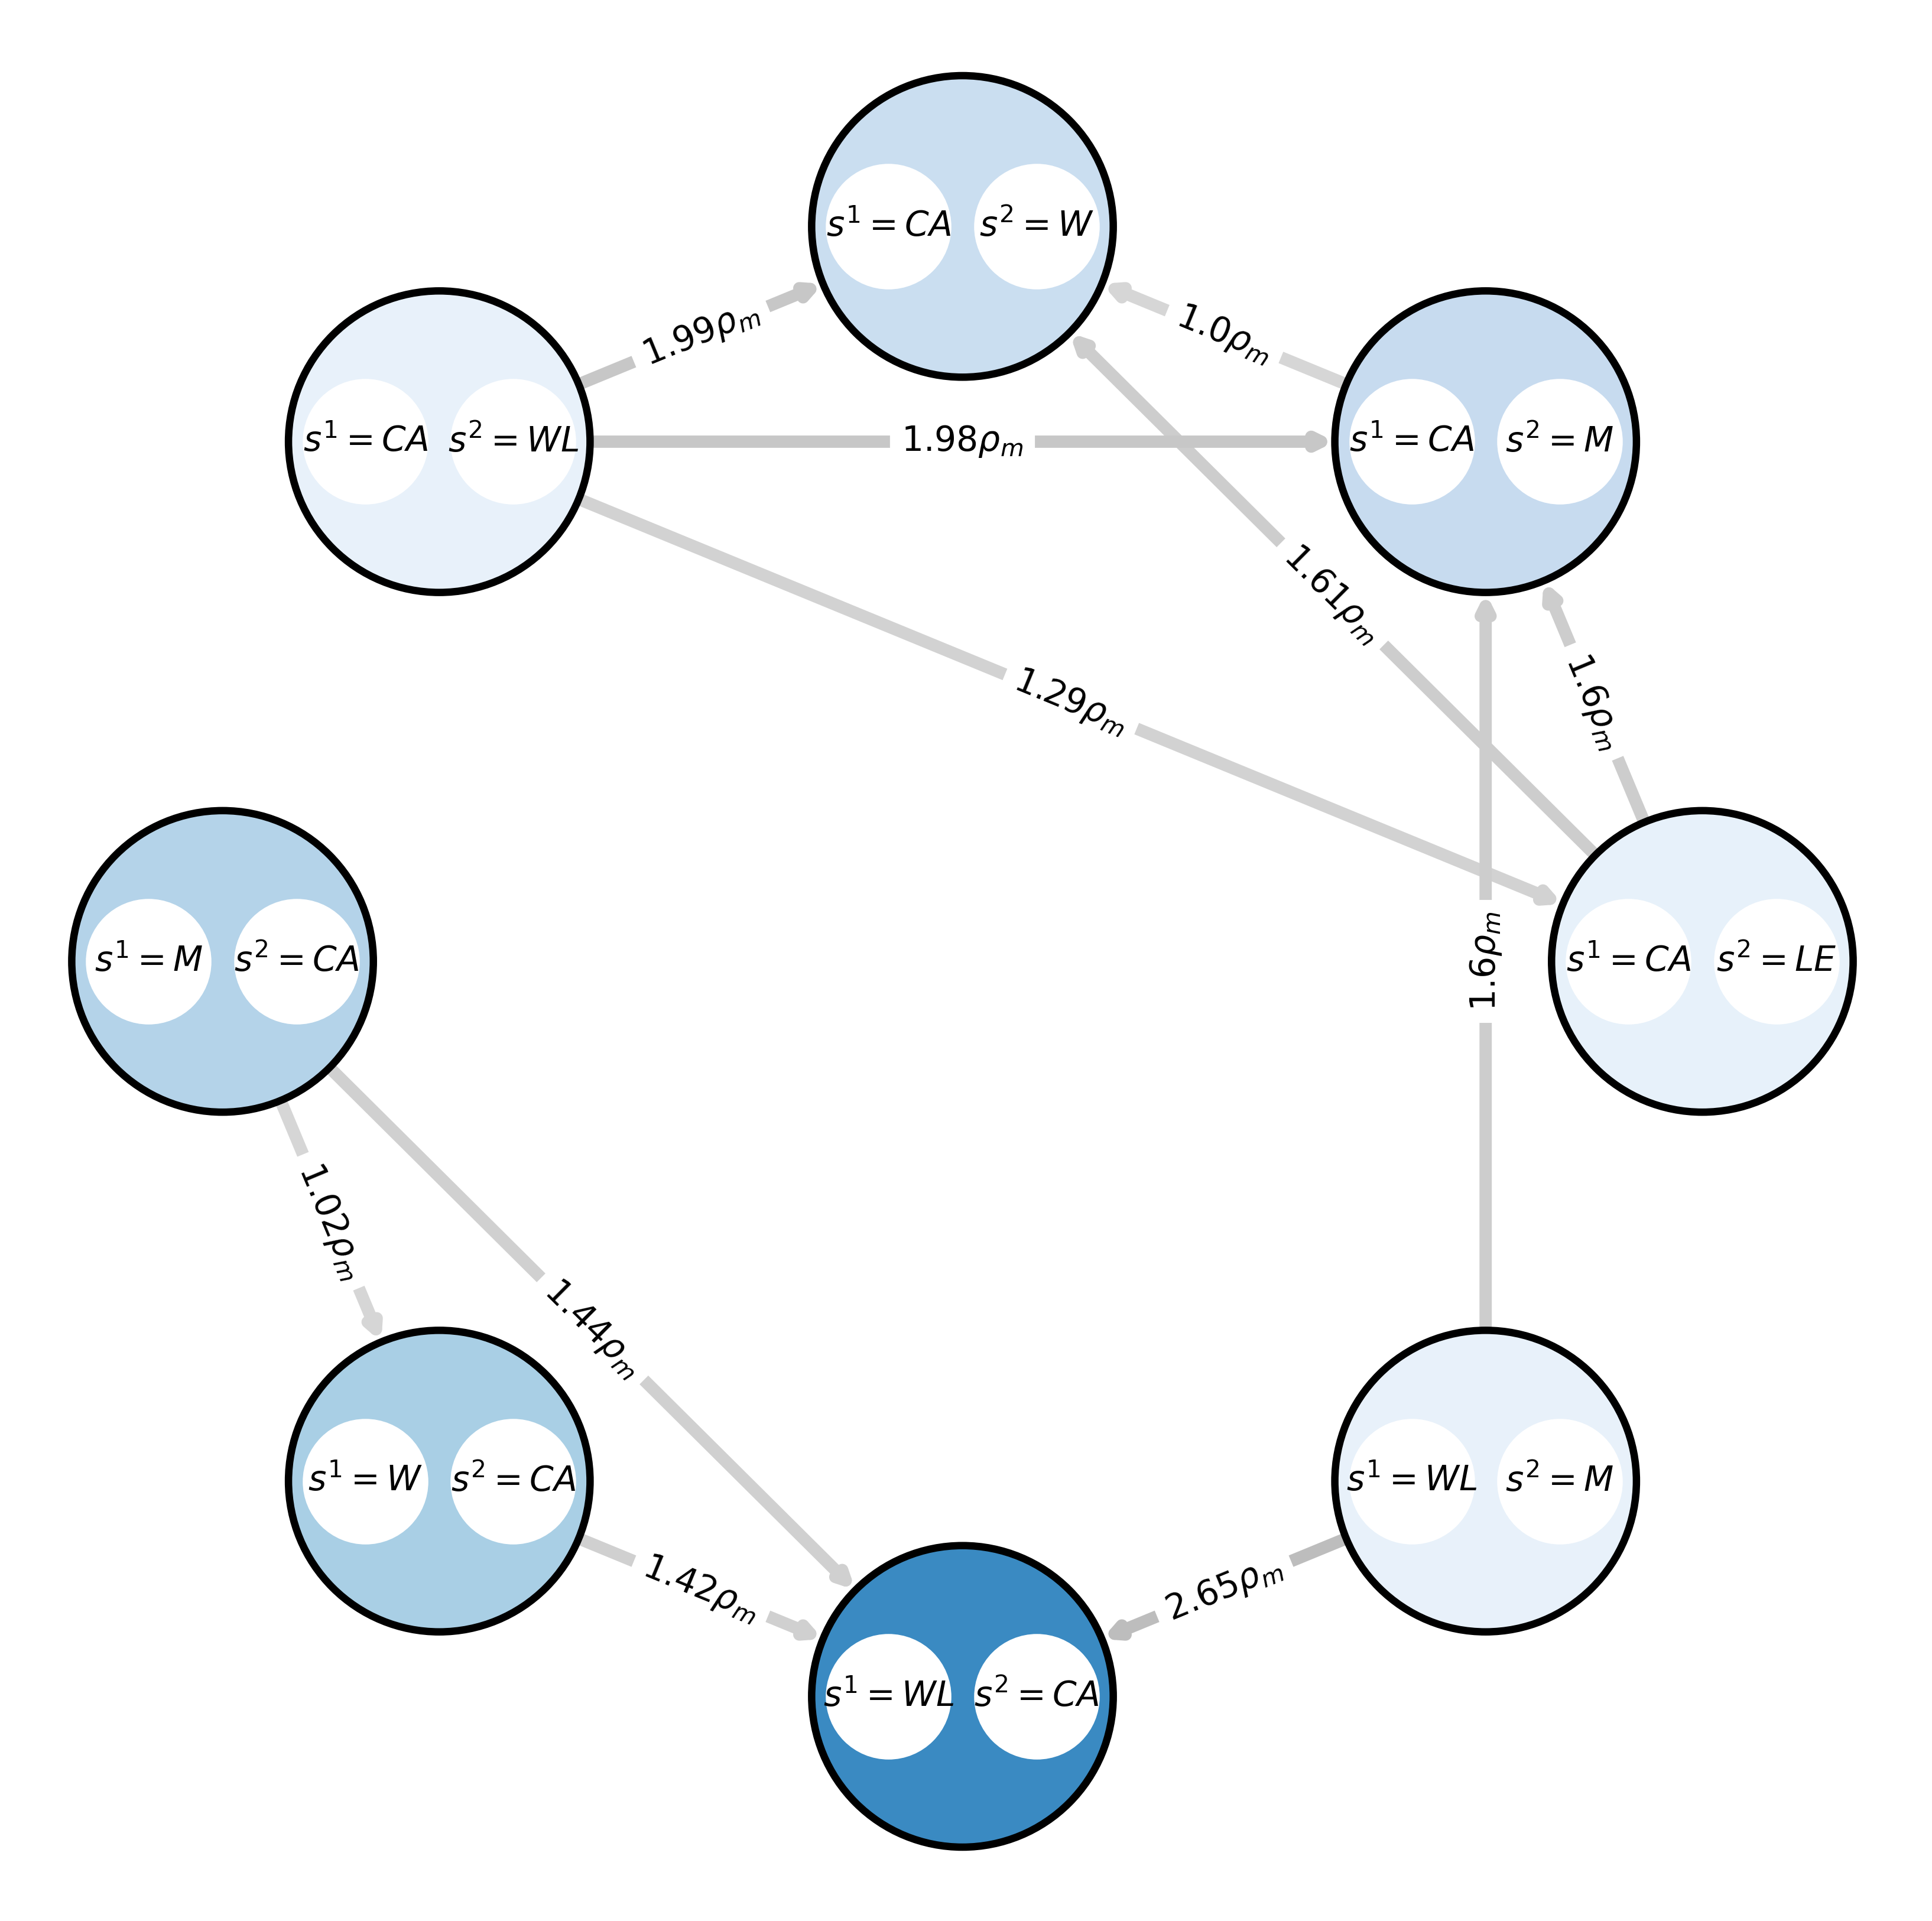
\includegraphics[width=\linewidth]{images/rg_1.3.png}
                \caption{$alpha=1.3$}
                \label{fig:response_graph_1.3}
            \end{subfigure}

            \begin{subfigure}[b]{0.45\linewidth}
                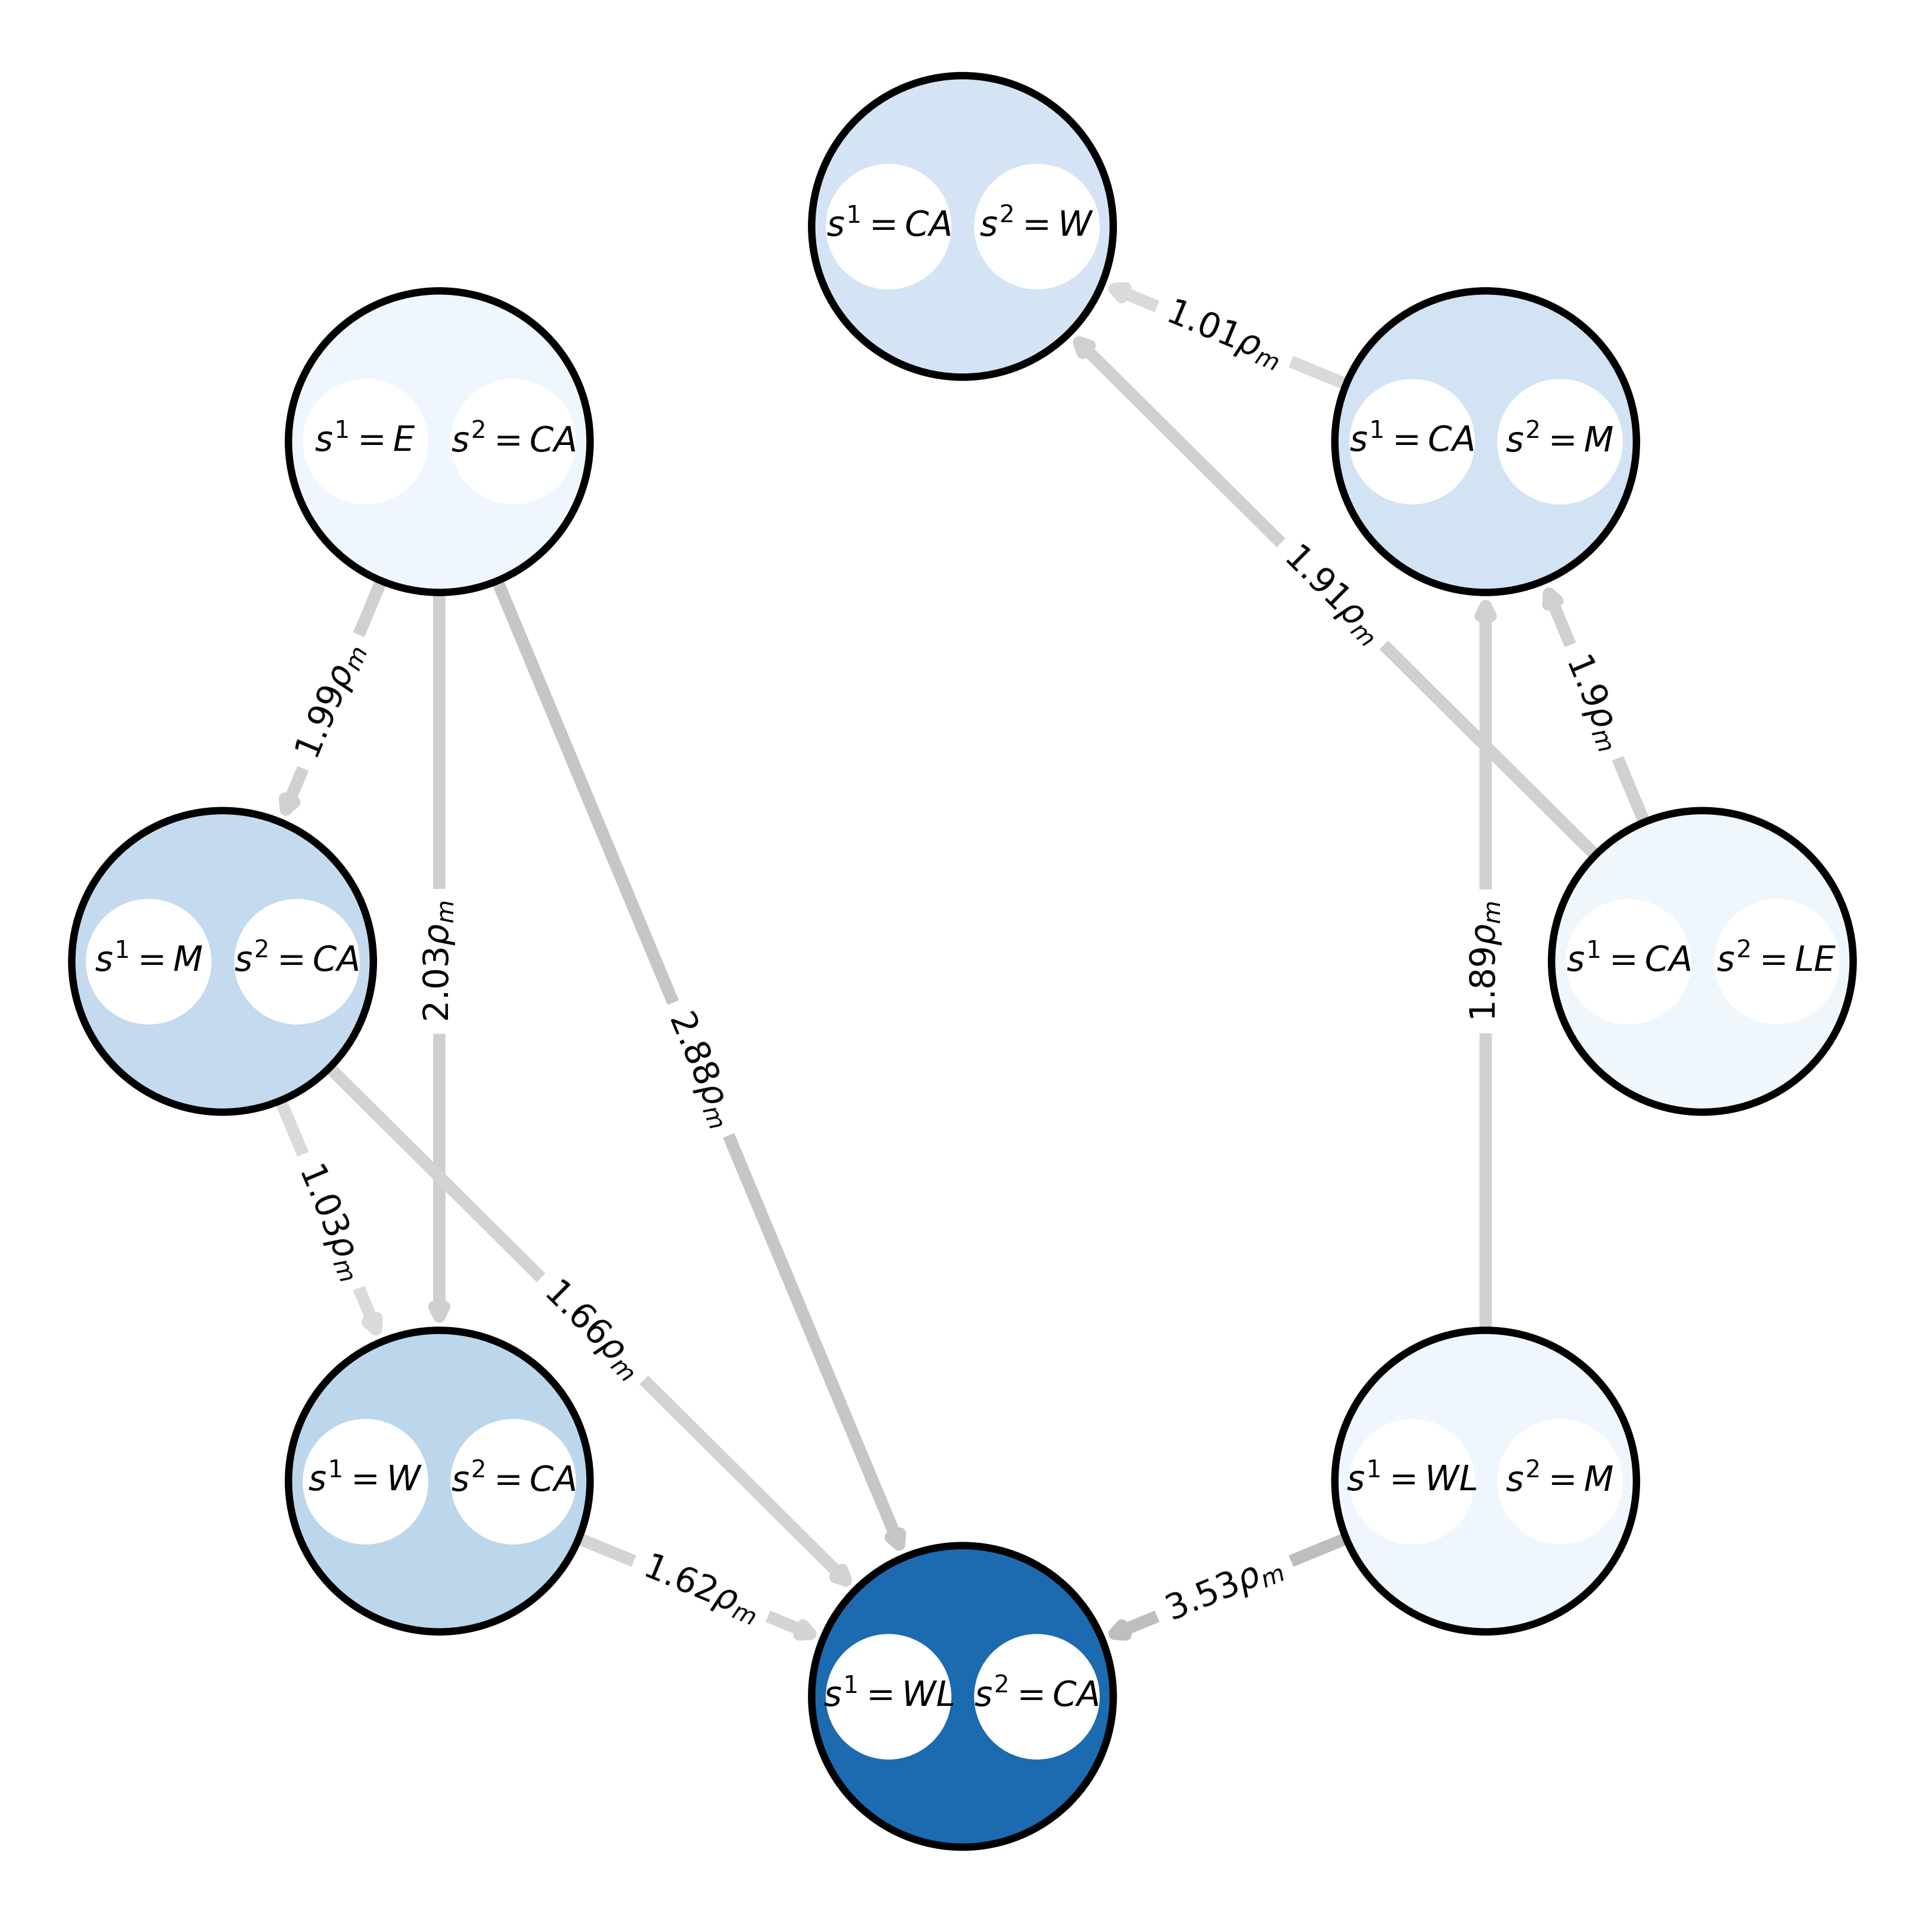
\includegraphics[width=\linewidth]{images/rg_1.9.png}
                \caption{$alpha=1.9$}
                \label{fig:response_graph_1.9}
            \end{subfigure}
            \hfill
            \begin{subfigure}[b]{0.45\linewidth}
                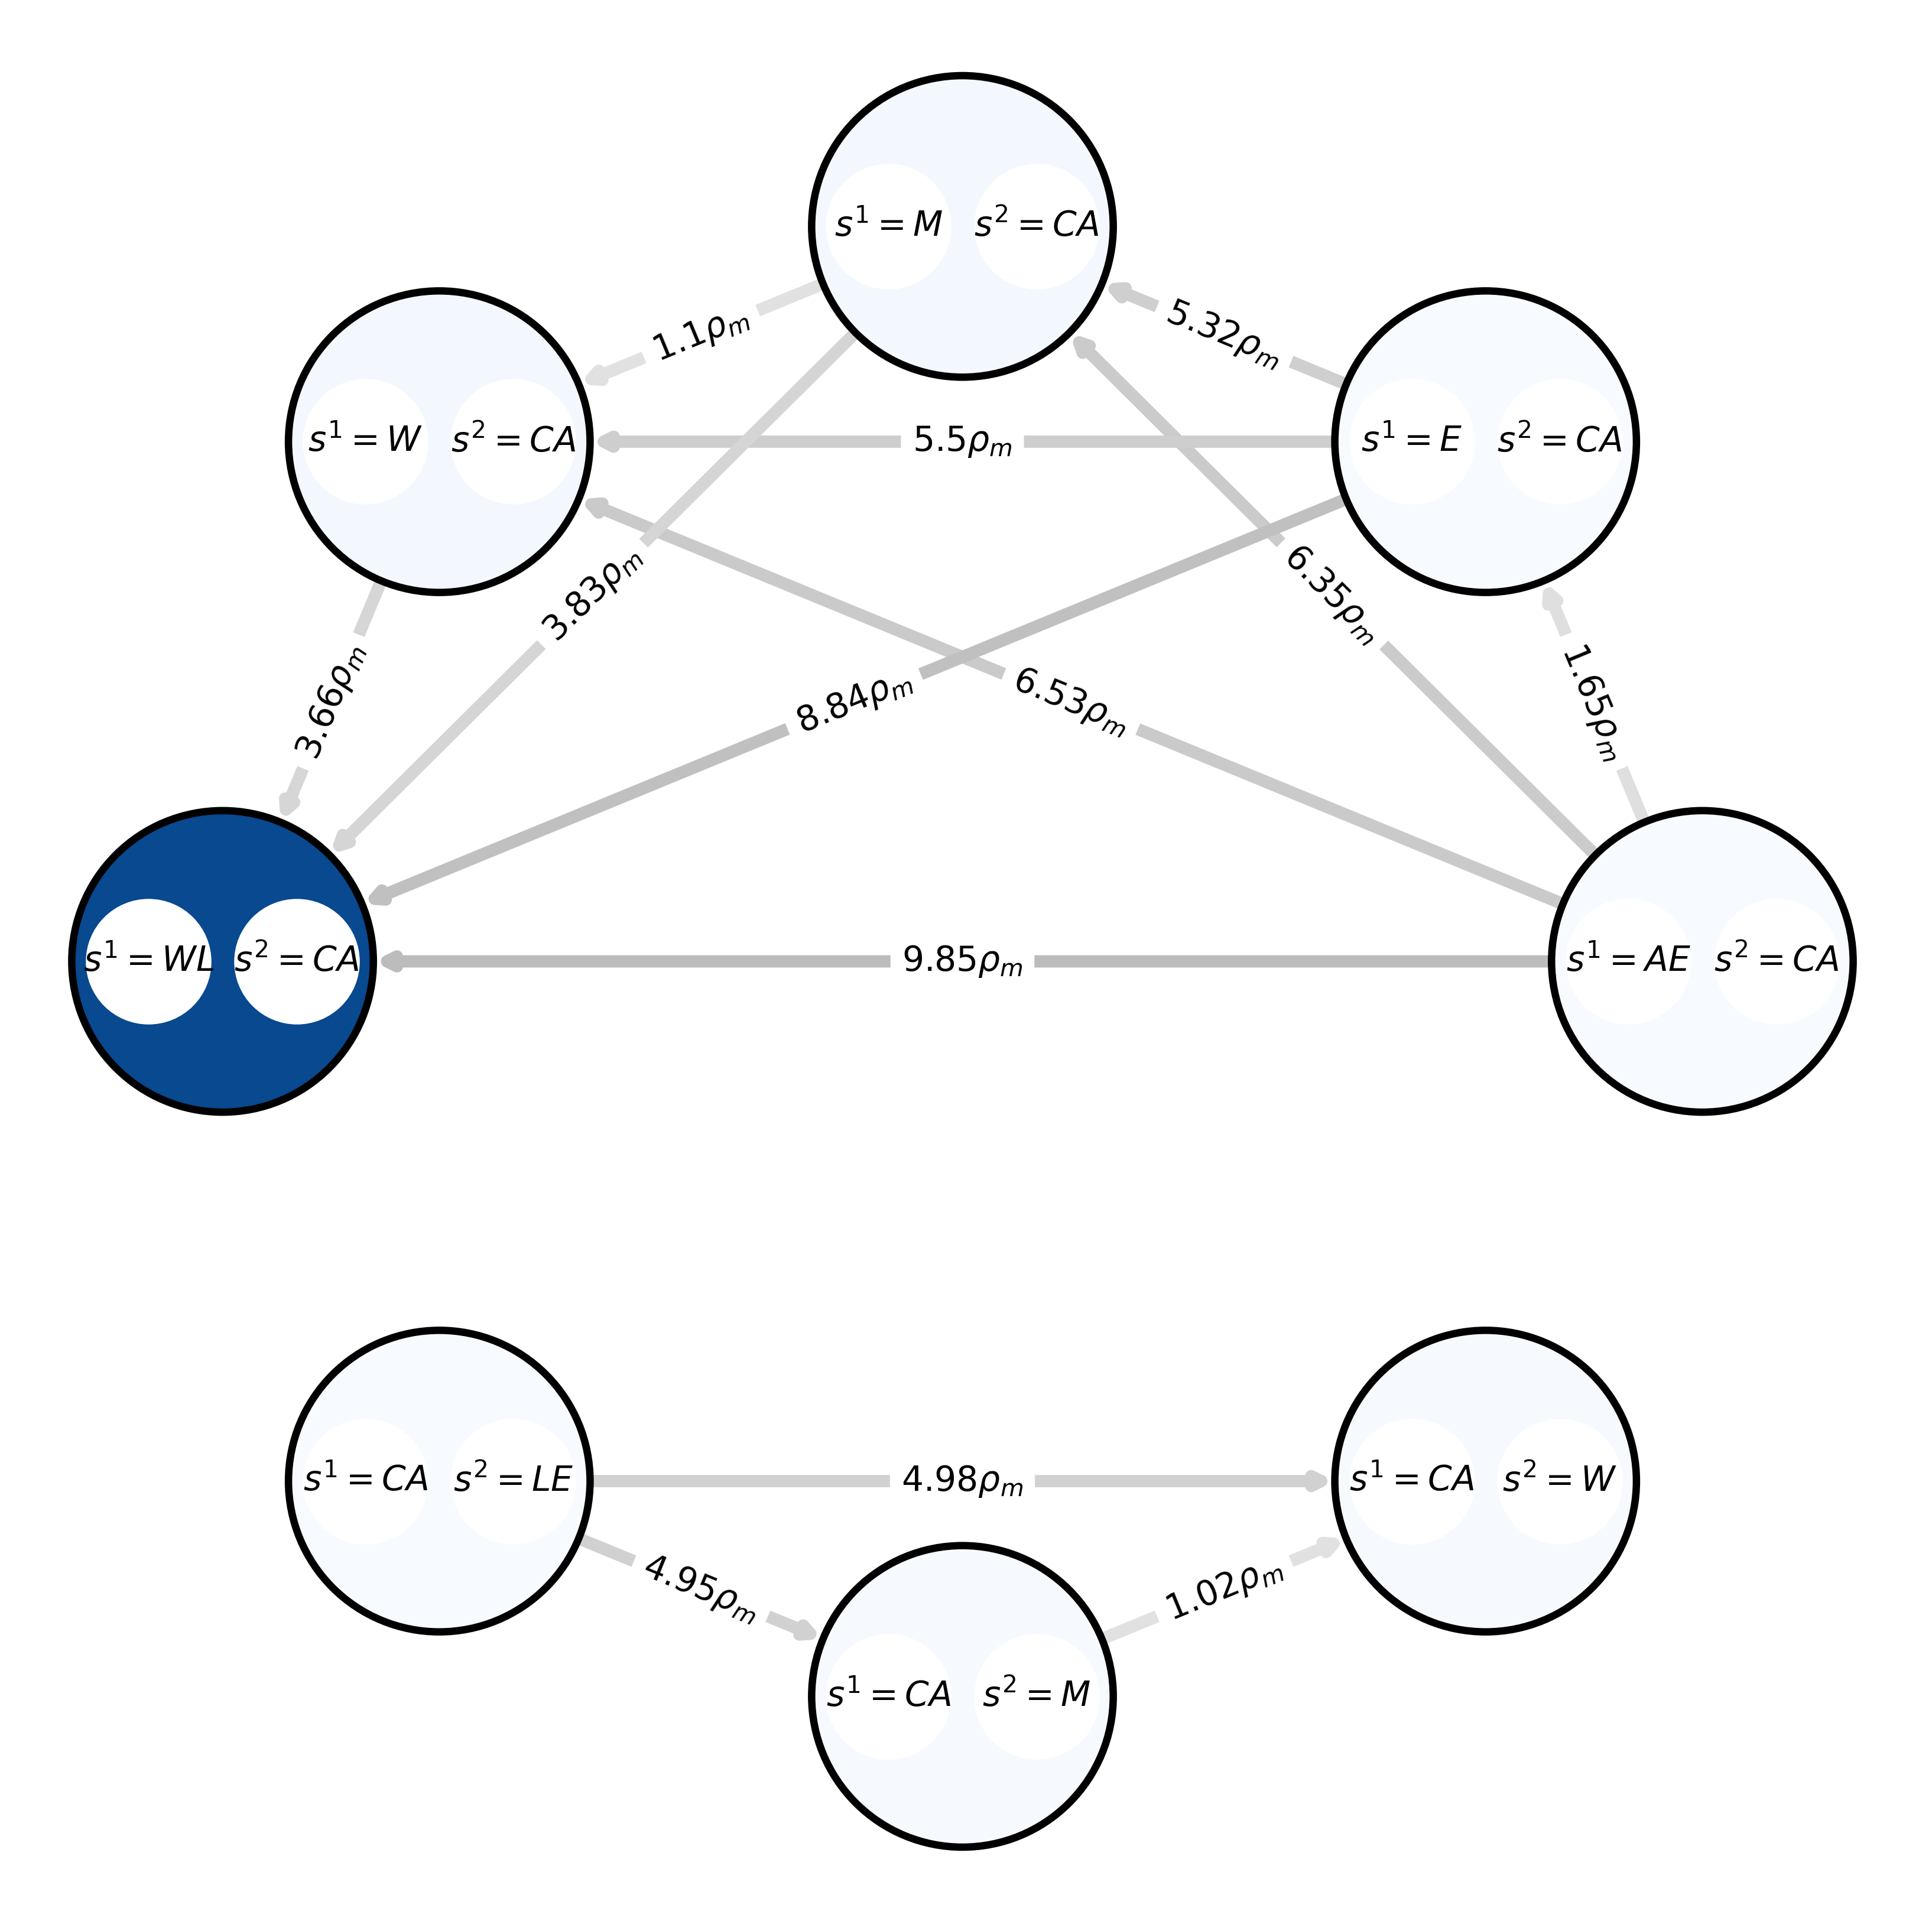
\includegraphics[width=\linewidth]{images/rg_6.4.png}
                \caption{$alpha=6.4$}
                \label{fig:response_graph_6.4}
            \end{subfigure}

            \caption{Response graphs of strategy profiles' dynamics.}
            \label{fig:response_graphs}
        \end{figure}
        %

        \noindent
        The response graph provides a visualization to interpret the \emph{$\alpha$-Rank} results. This graph illustrates the MCC, using the strategy profiles' masses from the stationary distribution, $\pi$, along with the fixation probability function $\rho$ provided by \emph{$\alpha$-Rank}. Figure~\ref{fig:response_graphs} shows the response graphs for $\alpha = 0.4$, $1.3$, $1.9$ and $6.4$. We consider it to be part of the descriptive framework $\mathcal{D}$, as it offers insights into how rankings were derived.\tinydouble

        \noindent
        Each node in the graph represents a unique strategy profile in the MCC, while the edges indicate transitions between them. The values on the edges show the fixation probabilities normalized by the neutral fixation probability, denoted as $\rho_m$. The nodes and edges are color-coded. Darker blue nodes represent more strong joint profiles, while lighter blue nodes represent transient ones. Similarly, bold arrows suggest a strong advantage in shifting between the nodes, whereas faint ones suggest less of an advantage.\tinydouble

        \noindent
        The response graph describes the overall dynamics of the strategy profiles in the empirical game. One prominent feature is the primary component of the MCC, specifically the profile (WL, CA). This profile, indicated by a dark blue color, has multiple graph edges leading to it, while none from it, indicating that strategies in this profile are non-transient. This is further supported by the large fixation probabilities along the edges. A particularly prominent example is the cluster (CA, LE)-(CA, M)-(CA, W), which consists of three strongly connected profiles, indicating that once a player adopts one of these profiles, they will likely remain within their cluster. These components reflect stable regions in the game’s strategy dynamics, where transitions between profiles become locked into a cycle.\tinydouble

        \noindent
        To further investigate the effect of $\alpha$ on profile dominance, we plotted the stationary distribution $\pi$ across all $\alpha$ values used in the experiments, for the top-performing strategy profiles (see Figure~\ref{fig:alpha_x_pi}). This visualization —also part of $\mathcal{D}$— helps us understand how the stationary distribution changes as the selection intensity increases. The x-axis represents the different $\alpha$ values, ranging from $0.1$ to $3$ in Figure~\ref{fig:alpha_x_pi_3}, and from $0.1$ to $10$ in Figure~\ref{fig:alpha_x_pi_10}, while the y-axis in both figures shows the mass of each strategy profile in the stationary distribution $\pi$. As $\alpha$ increases, the distribution converges, indicating that the selection process stabilizes. The final mass distributions are highlighted in boxed regions. The legend on the right side of the plot displays the top-performing joint strategies, with the stronger ones appearing at the top.
        %
        \begin{figure}[H]
            \centering
            \begin{subfigure}[b]{0.49\linewidth}
                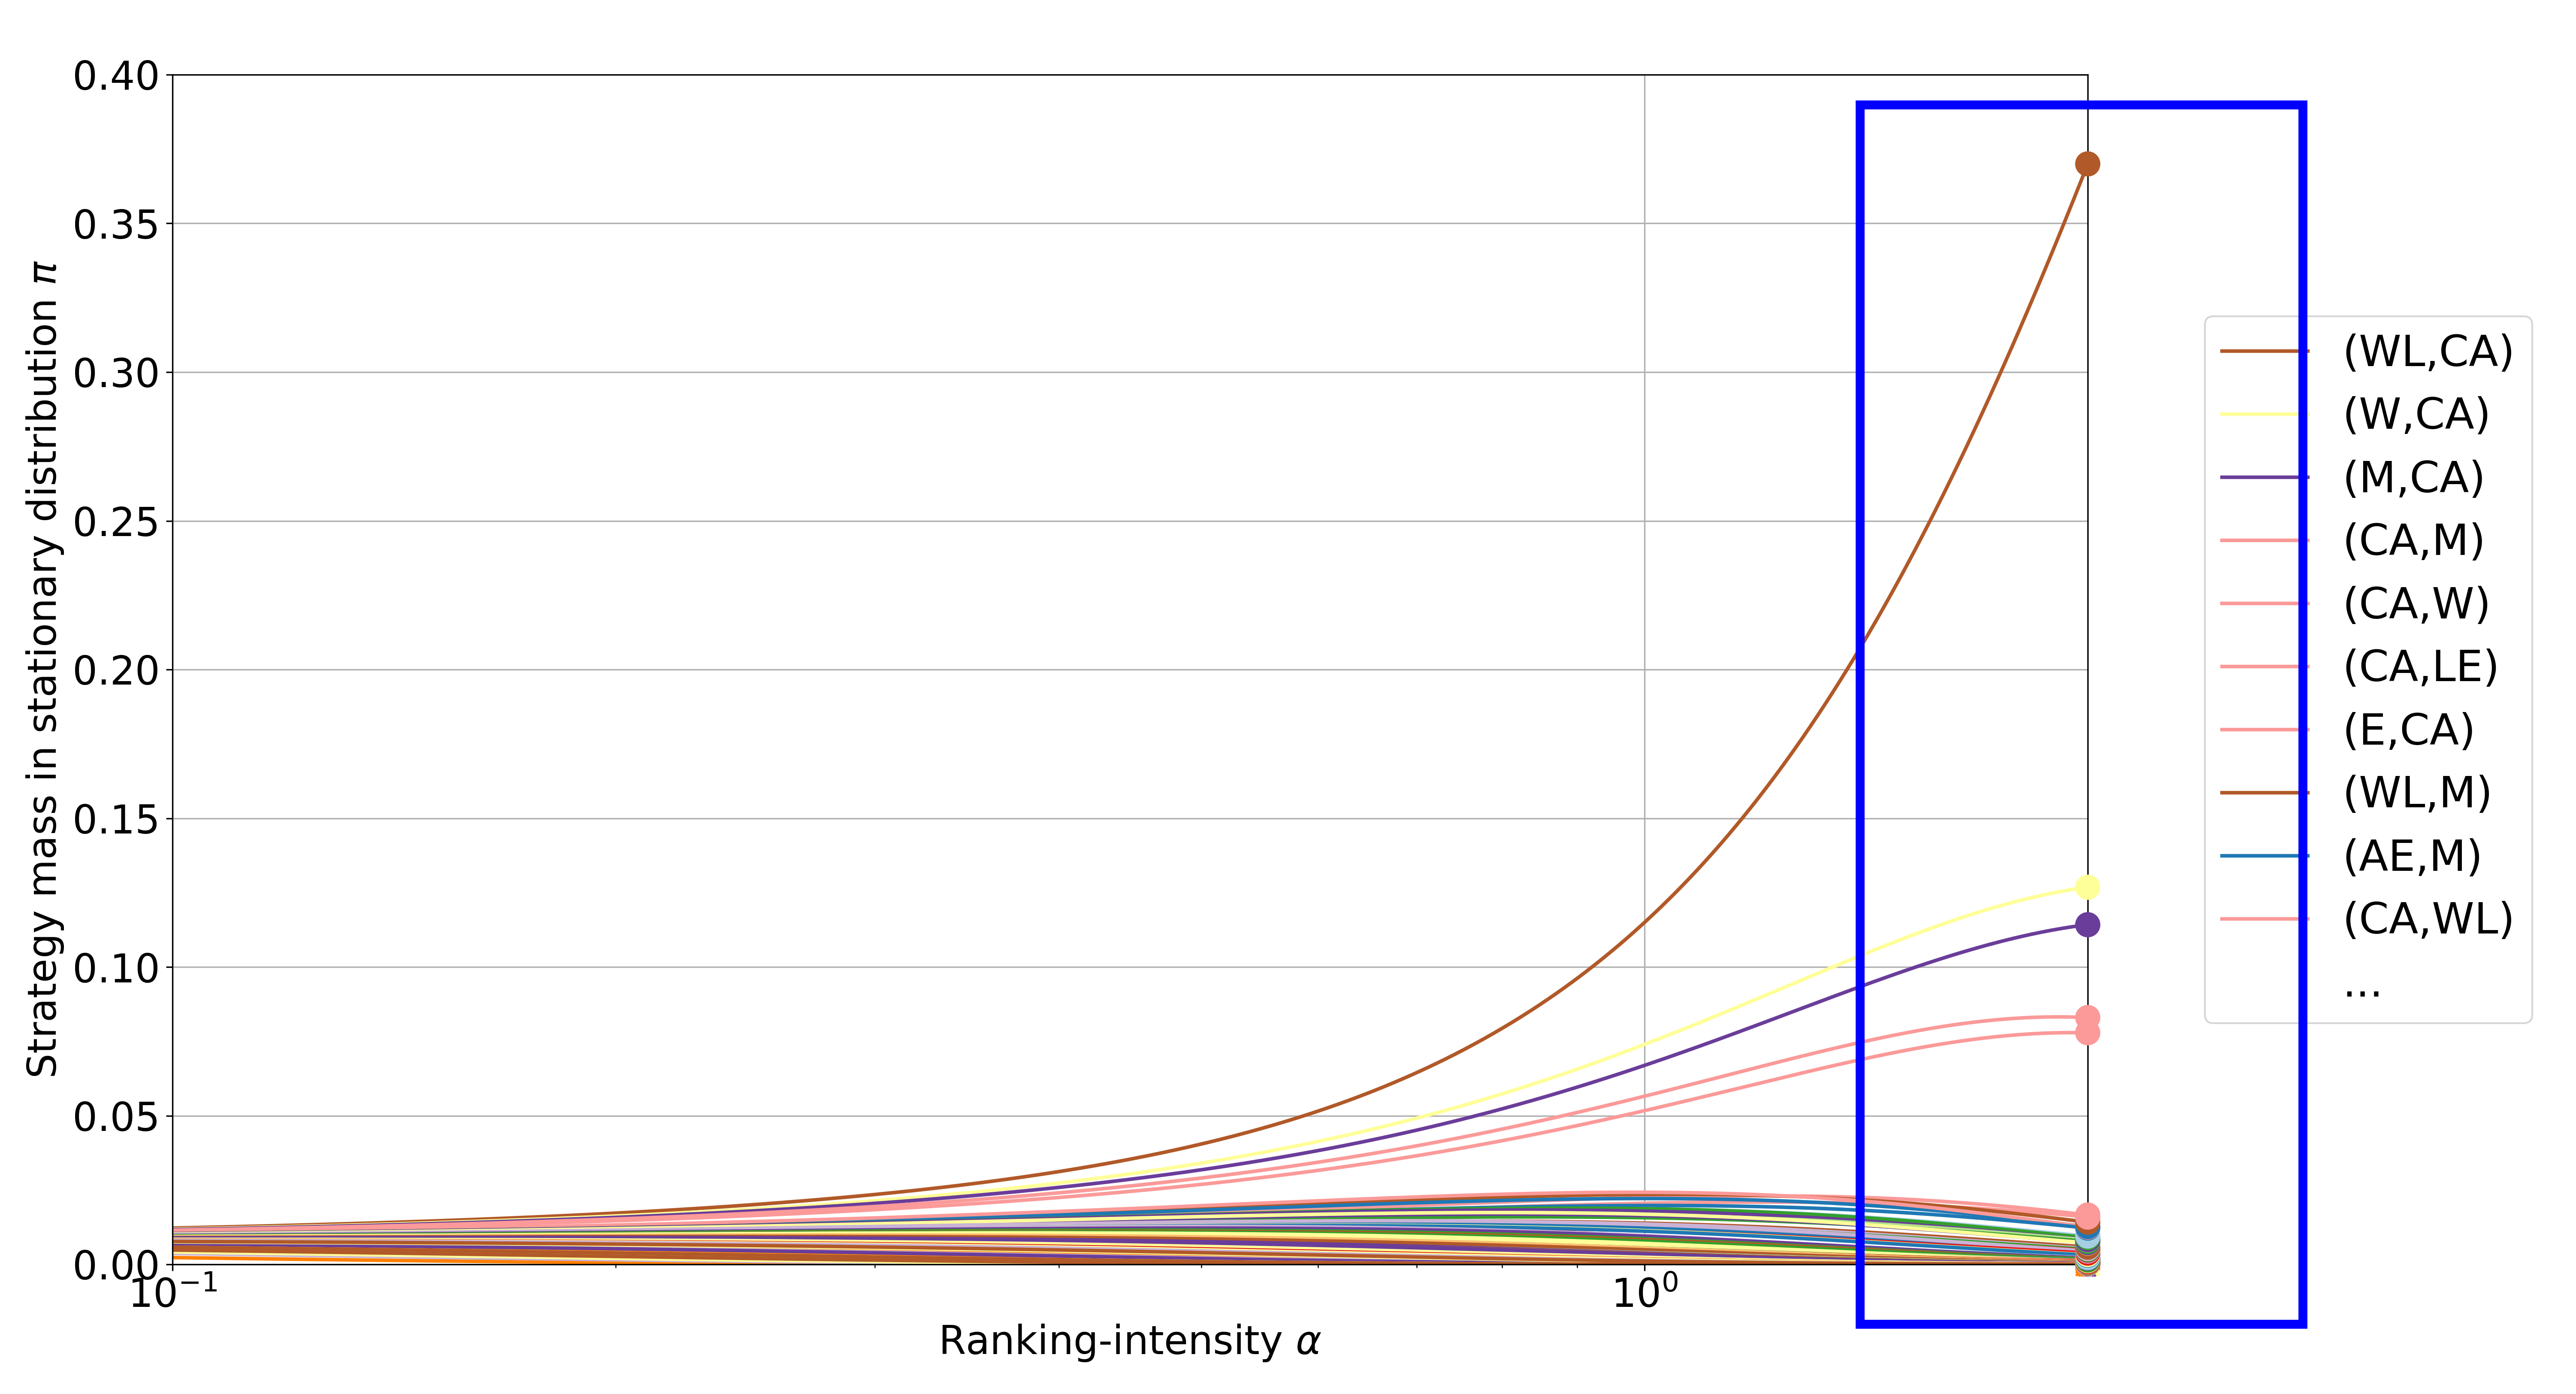
\includegraphics[width=\linewidth]{images/alpha_x_pi_3.png}
                \caption{Mass across $\alpha \in [0.1, 3]$.}
                \label{fig:alpha_x_pi_3}
            \end{subfigure}
            \hfill
            \begin{subfigure}[b]{0.49\linewidth}
                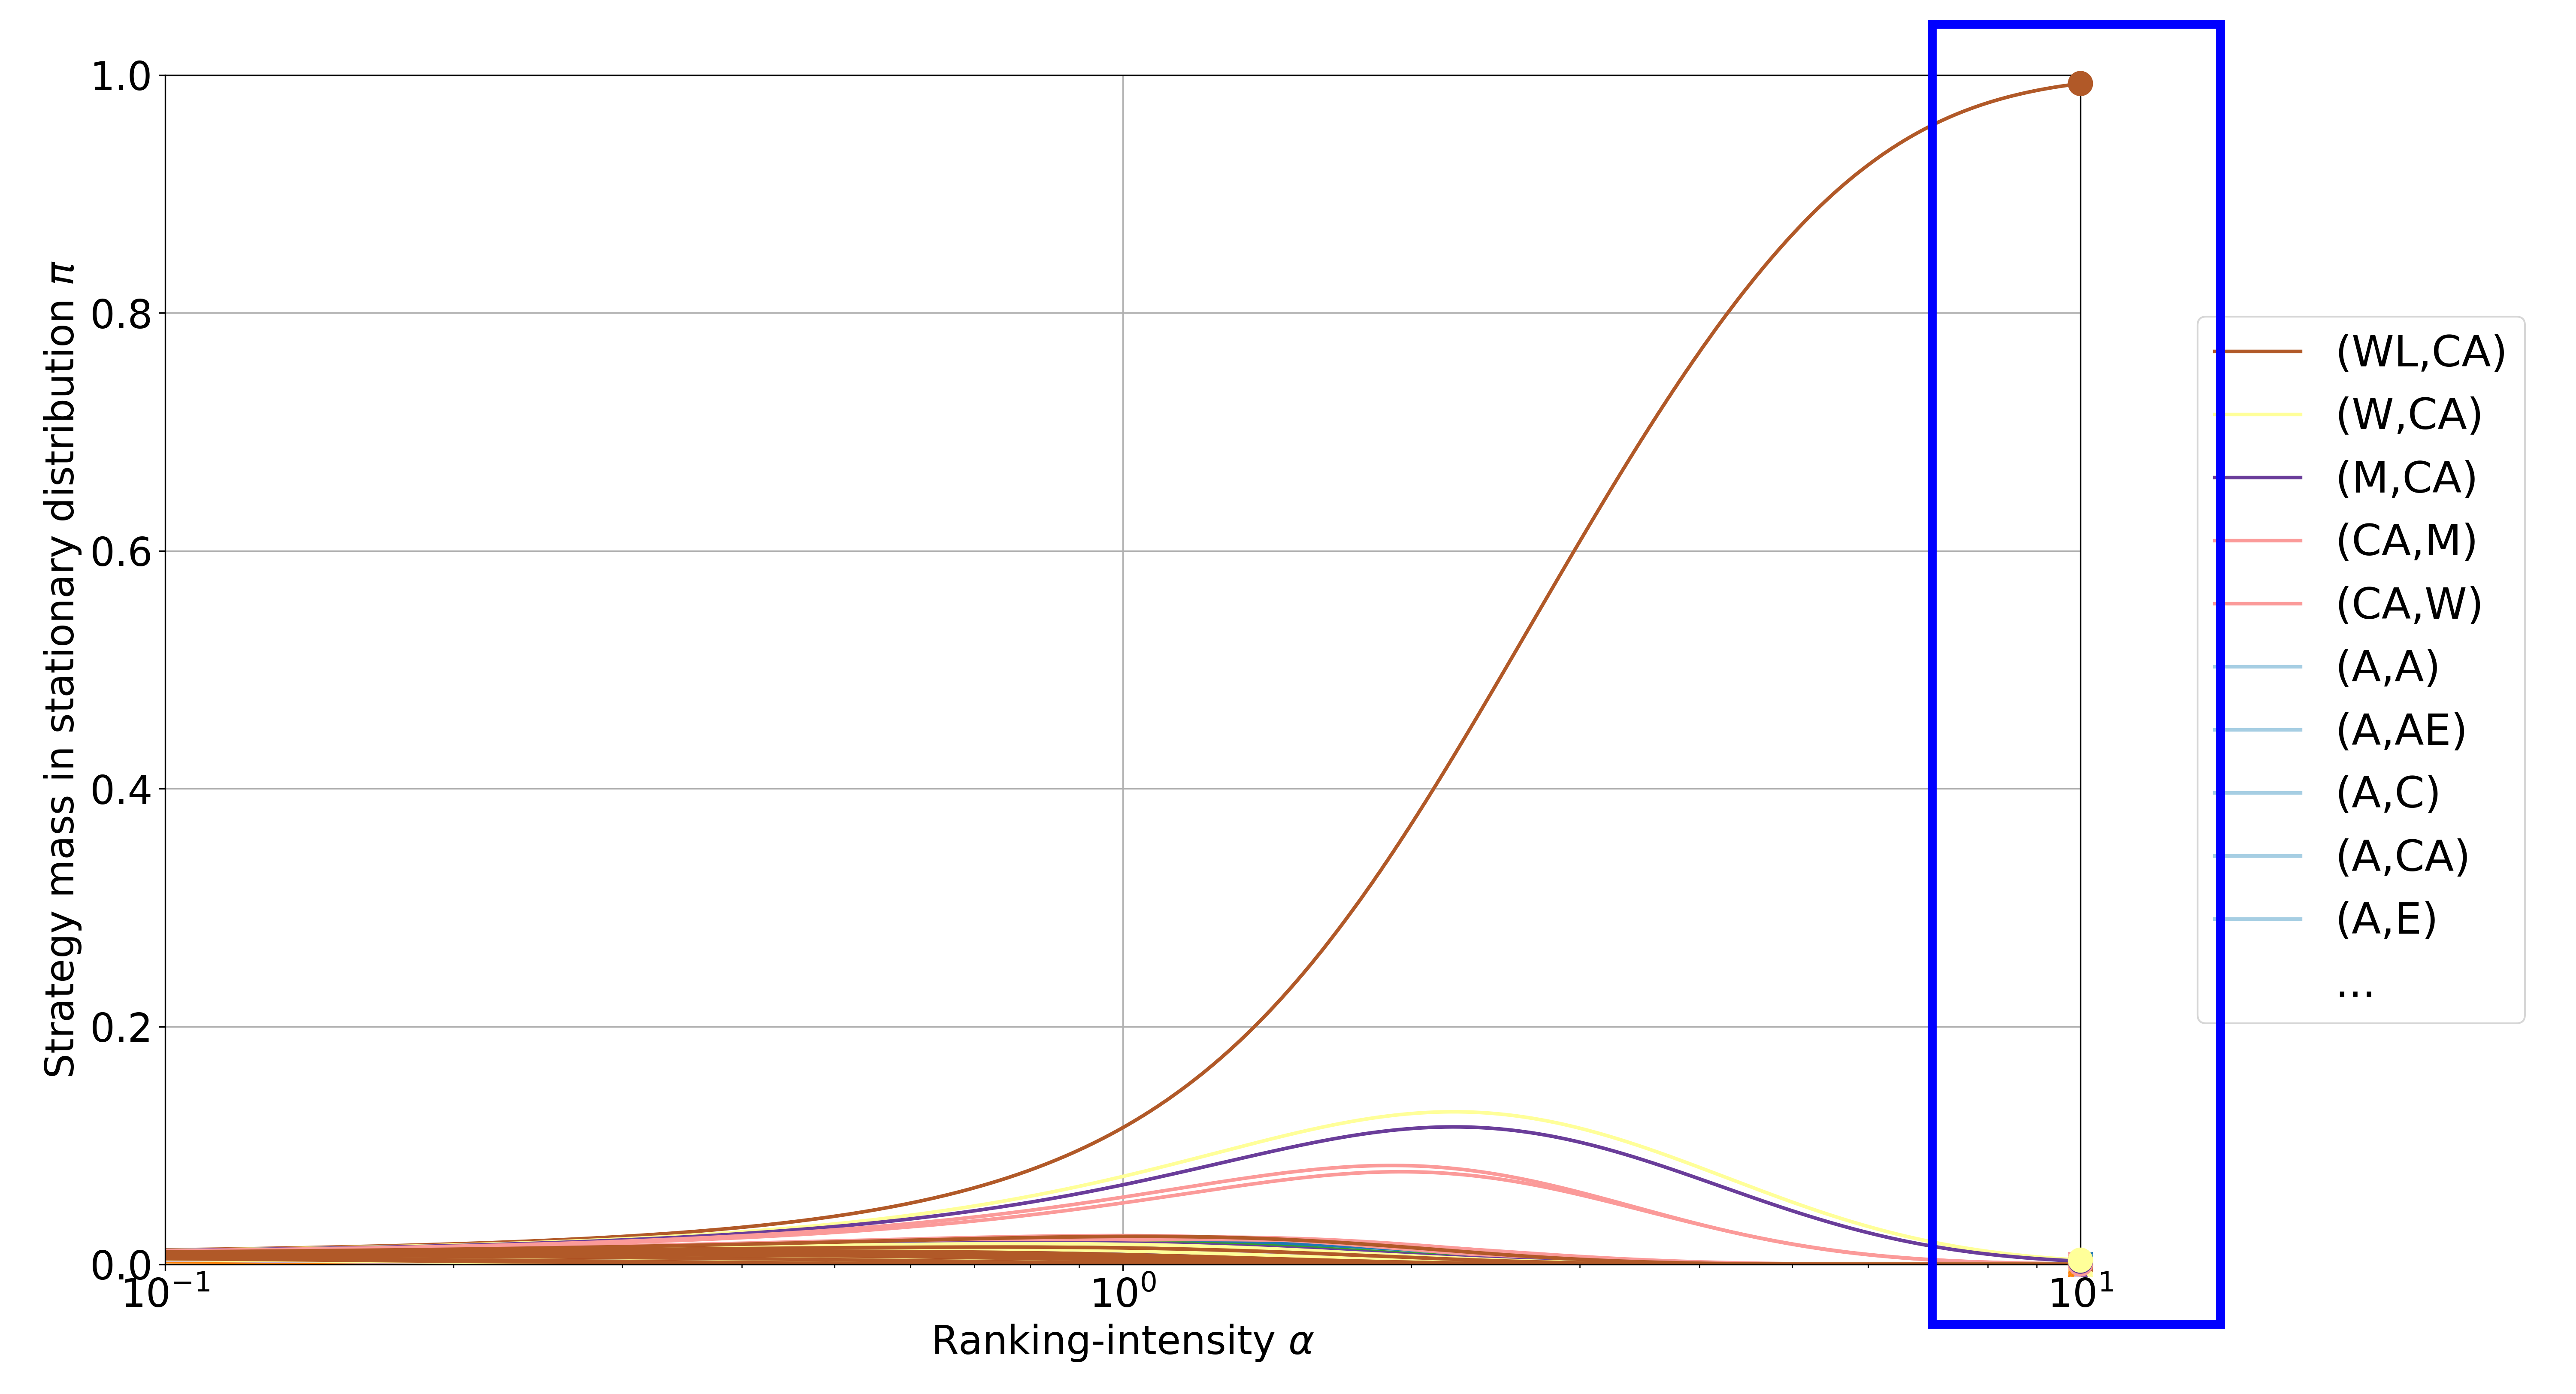
\includegraphics[width=\linewidth]{images/alpha_x_pi_10.png}
                \caption{Mass across $\alpha \in [0.1, 10]$.}
                \label{fig:alpha_x_pi_10}
            \end{subfigure}
            \caption{Effect of ranking intensity $\alpha$ on strategy profile mass in the stationary distribution $\pi$.}
            \label{fig:alpha_x_pi}
        \end{figure}
        %

        \noindent
        We plot two such graphs to observe how the mass of strategy profiles is distributed in the MCCs across different $\alpha$ values. In the stationary distribution resulting from a bigger $\alpha$, the dominant strategy profile (WL, CA) in the MCC achieves a mass of 1, with all other profiles dropping to 0. This is clearly illustrated in the second plot (see Figure~\ref{fig:alpha_x_pi_10}). However, regarding the mass distribution for a smaller range of $\alpha$, depicted n the first plot, the game has not yet converged to the final MCC.

\newpage
\subsection{Conclusion}

    In this study, we developed a methodology for identifying strong joint-strategies in dynamic multi-agent games, accounting for stability and performance, using the \emph{$\alpha$-Rank} evolutionary algorithm. The methodology is applied on a stochastic version of the \emph{Graph Coloring Problem}, in which players work together to color a graph while ensuring that neighboring vertices are assigned different colors. According to the methodology, first we transformed the game into its empirical form, by defining strategies (styles of play). We then designed and trained Deep Q-Learning policy models that realize those styles of play in the underlying game, and run simulations to generate the empirical payoff matrix. \emph{$\alpha$-Rank}, applied to this matrix, results into a unique stationary distribution over strategy profiles that defines the empirical game's MCC. The \emph{$\alpha$-Rank} not only helped us identify stable strategy profiles resistant to changes but also provided a descriptive framework for understanding why certain profiles prevail in the long run, based on the underlying dynamics of the game. Through this approach, we successfully described a concise methodology for evaluating and ranking agents' joint policies, considering their long-term interactions in dynamic settings, while also explaining how strategy profiles are defined within the MCC.\tinydouble

    \noindent
    Future work involves (a) applying the methodology in more complex and large-scale settings, accounting for strategy profiles of multiple stakeholders that may collaborate and/or compete, (b) using machine learning methods to identify different styles of play from demonstrations and specifying the empirical game, (c) exploring advanced models able to adapt their strategies based on observed behaviors based on the behavior of co-players, and (d) applying the methodology into real-world settings where agents need to align with human preferences in dynamic settings.

\newpage